\documentclass[letter]{beamer}
%removed: handout (ignores "animations")

\usepackage[utf8]{inputenc}
\usepackage{graphicx}
\usepackage{minted}

\usetheme{AnnArbor}
%\usetheme{CambridgeUS}
\usecolortheme{beaver}

\title[IIC2333] % (optional, only for long titles)
{02 - Administración de Memoria}
\subtitle{IIC2333 - Sistemas Operativos y Redes}
\author[C.Ruz] % (optional, for multiple authors)
{Cristian Ruz -- {\tt cruz@ing.puc.cl} }
\institute[PUC] % (optional)
{
  Departamento de Ciencia de la Computación\\
  Pontificia Universidad Católica de Chile
}
\date[2/2015] % (optional)
{Semestre 2-2015}
%\subject{Informatik}

\AtBeginSection[]
{
  \begin{frame}
    \frametitle{Contenidos}
    \tableofcontents[currentsection]
  \end{frame}
}

\begin{document}

%---------------------------------------------------------------------
\frame{\titlepage}

%---------------------------------------------------------------------
\begin{frame}
\frametitle{Contenidos}
%\tableofcontents[currentsection]
\tableofcontents
\end{frame}


%---------------------------------------------------------------------
\section{Direccionamiento de Memoria}

\subsection{Funcionamiento básico}

\begin{frame}
  \frametitle{Memoria}

  ¿Definición? 
  \onslide<2->{
  \begin{block}{{\bf Memoria}}
    \begin{itemize}
      \item Un gran arreglo de {\em bytes}
      \item Cada uno con su propia {\bf dirección}
    \end{itemize}
  \end{block}
  }
  
  \onslide<3->{¿Para qué? \ldots} \onslide<4->{¡para todo!}
  
  \begin{itemize}
    \item <4-> PC lee instrucciones desde una dirección de memoria
    \item <4-> Instrucciones pueden requerir leer operaandos desde otra dirección de memoria
    \item <4-> Resultados suelen ser almacenados en alguna dirección de memoria
  \end{itemize}
  
  \onslide<4->{La unidad de memoria ve un flujo de solicitudes de lectura + escritura}
  
    
  
\end{frame}

%---------------------------------------------------------------------
\begin{frame}
  \frametitle{Memoria}
  \framesubtitle{¿Cómo funciona?}

  Dos problemas: velocidad y protección
  
  {\bf Velocidad}
  
  \begin{itemize}
    \item {\bf Registros} suelen ser accedido en un ciclo de CPU
    \item {\bf Memoria} debe ser accedida a través de solicitud al {\bf bus de memoria}
      \begin{itemize}
        \item Varios ciclos de espera
        \item Caché como unidad de memoria intermedia de rápido acceso
      \end{itemize}
  \end{itemize}

  {\bf Protección}
  
  \begin{itemize}
    \item Procesos no deben poder acceder memoria de otros procesos
    \item Por cada acceso se debe verificar si está dentro de los límites
      \begin{itemize}
        \item Pero es lento si el S.O. debe intervenir en cada acceso
        \item Protección implementada por {\em hardware}
      \end{itemize}
  \end{itemize}
  

\end{frame}


%---------------------------------------------------------------------
\begin{frame}
  \frametitle{Memoria}
  \framesubtitle{Protección por {\em hardware}}

  Rango de direcciones {\em legales} por proceso

  \begin{columns}[c]
    \begin{column}[T]{6cm}
      Dos registros:
        \begin{itemize}
          \item {\bf Base}
          \item {\bf Límite}
        \end{itemize}
      Definidos para cada proceso
    \end{column}
    \begin{column}[T]{5cm}
      \begin{center}
        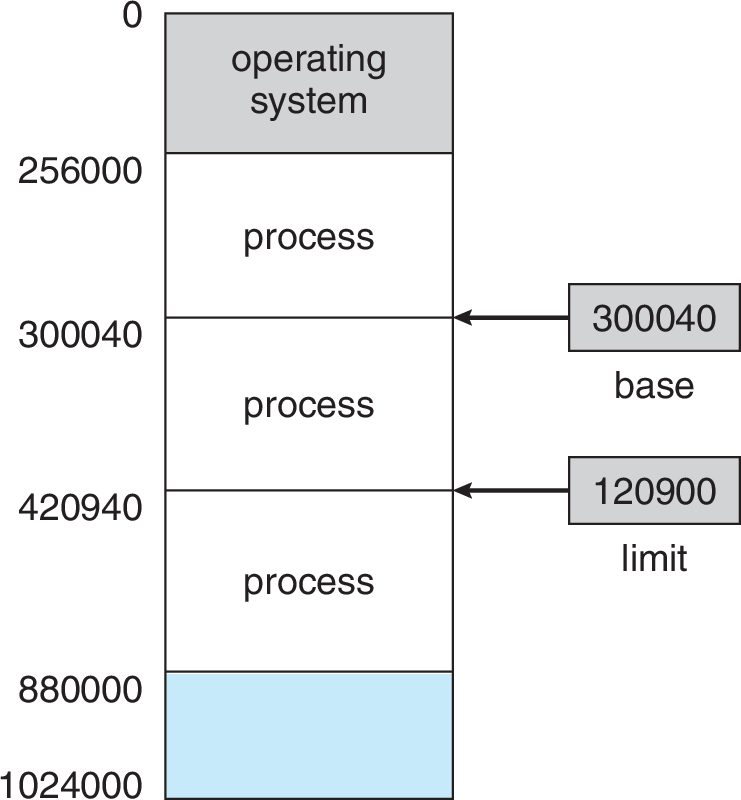
\includegraphics[width=5cm]{figs/02-8_01.pdf}
      \end{center}
    \end{column}
  \end{columns}
    

\end{frame}
%---------------------------------------------------------------------
\begin{frame}
  \frametitle{Memoria}
  \framesubtitle{Protección por {\em hardware}}

  Registro {\bf base} y {\bf limite} se cargan en registro de {\em hardware}.

  \begin{center}
    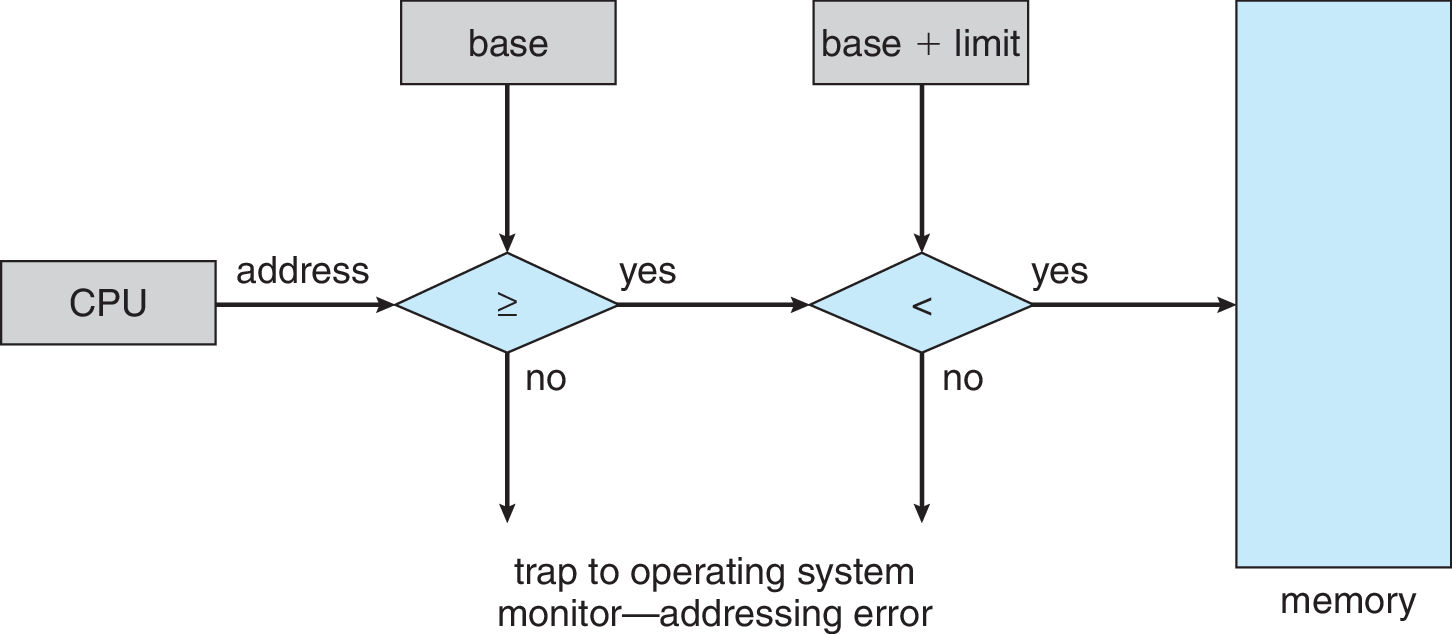
\includegraphics[width=10cm]{figs/02-8_02.pdf}
  \end{center}

  ¿En qué modo pueden modificarse estos registros? \onslide<2->{Sólo modo monitor}
  
\end{frame}

%---------------------------------------------------------------------
\begin{frame}
  \frametitle{Memoria}
  \framesubtitle{Asociación de direcciones ({\em address binding})}

  ¿Cómo saber a qué dirección acceder?
  
  \onslide<2->{
  Sistema Operativo {\em carga} un programa en memoria copiando su código
  a {\em alguna} sección de la memoria (¿secuencialmente?)
  }
  
  \onslide<3->{
  Instrucción de un programa:
  \begin{center}
    {\em Leer dirección 0x00F3}
  \end{center}
  }
  \onslide<4->{Sistema Operativo debe haber cargado el programa de la dirección 0x0000}
  
  \onslide<5->{¿Y si otro programa hace la misma solicitud?}
  
  \onslide<6->{Compiladores no escriben (casi nunca) direcciones absolutas:
  
  \begin{center}
    {\em Leer dirección F3 posiciones desde el inicio}
  \end{center}
  }
  
\end{frame}
%---------------------------------------------------------------------
\begin{frame}
  \frametitle{Direccionamiento}
  \framesubtitle{¿Cuándo se hace la asociación?}

  \begin{columns}[c]
    \begin{column}[T]{8cm}
      En alguna de estas etapas:
      \begin{itemize}
        \item {\bf Tiempo de compilación} ({\em Compile time}).
              Requiere conocer dónde será cargado el programa. Si eso cambia se debe recompilar.
              Ej: programas MS-DOS.
        \item {\bf Tiempo de carga} ({\em Load time}).
              Código generado debe ser {\em relocalizable}. Una vez que se carga, la dirección queda fija.
        \item {\bf Tiempo de ejecución} ({\em Execution time}, {\em Run time}).
              Permite que el proceso sea sacado y regresado a distintos sectores de memoria.
      \end{itemize}
    \end{column}
    
    \begin{column}[T]{3.5cm}
      \begin{center}
        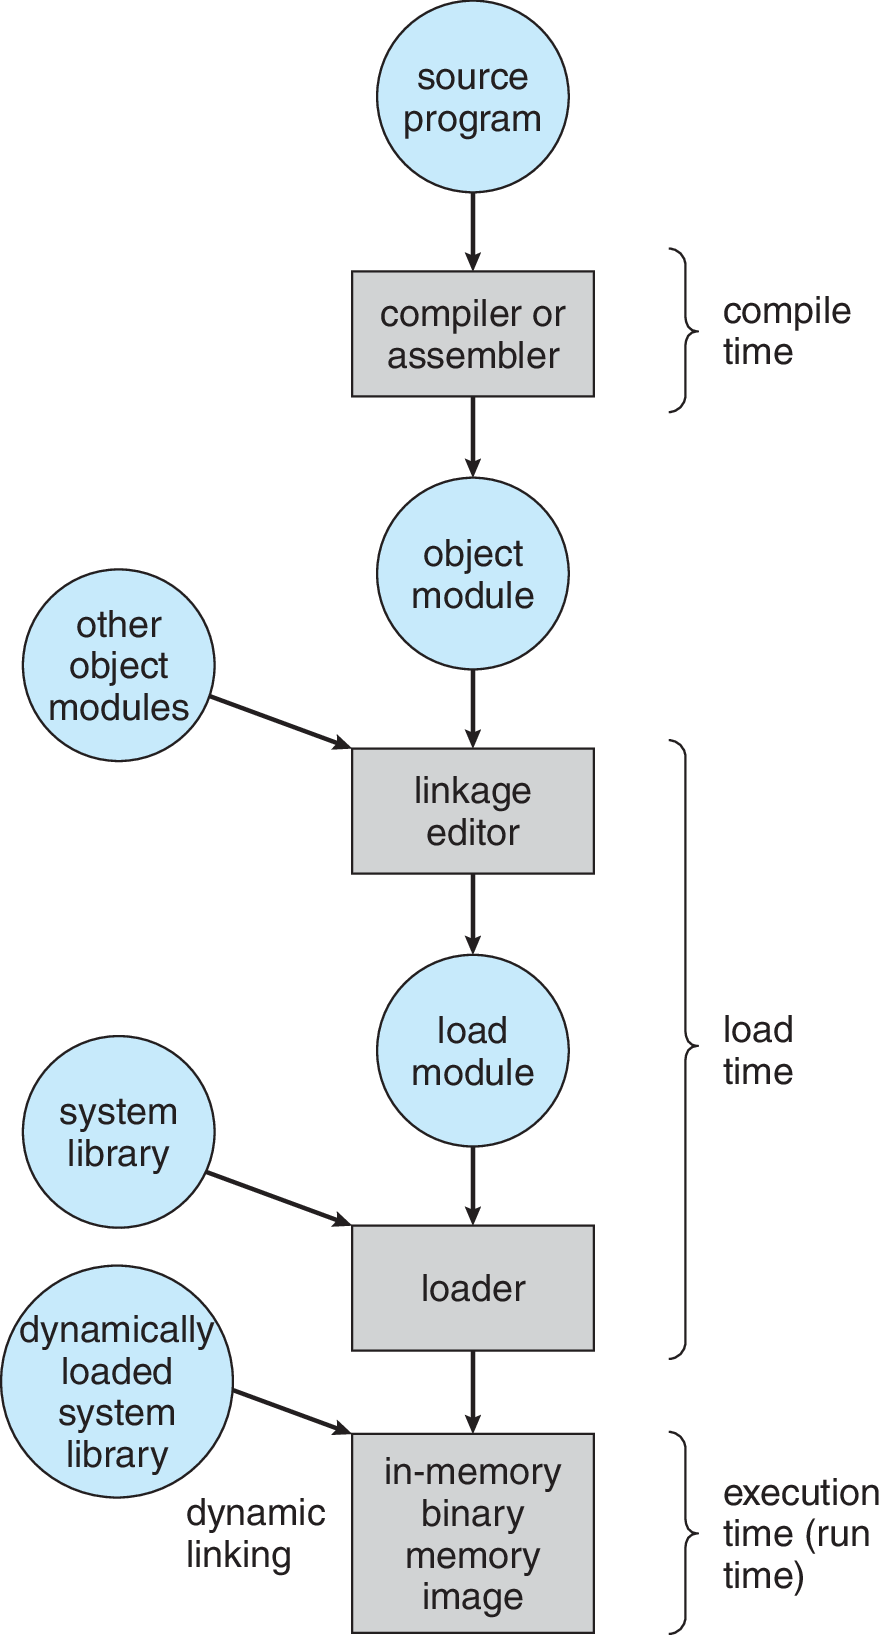
\includegraphics[width=3cm]{figs/02-8_03.pdf}
      \end{center}
    \end{column}
  \end{columns}


\end{frame}

%---------------------------------------------------------------------
\begin{frame}
  \frametitle{Direccionamiento}
  \framesubtitle{Direcciones física y lógicas}

  Dirección solicitada por CPU: {\bf dirección lógica}
  
  Dirección recibida por memoria: {\bf dirección física}
  
  \onslide<2->{¿Qué pasa entre medio? \ldots depende de la etapa de generación}

  \begin{itemize}
    \item <3-> Tiempo de compilación y carga $\to$ direcc. lógica == física
    \item <4-> Tiempo de ejecución $\to$ conversión vía {\em memory management unit}
  \end{itemize}

  \begin{center}
    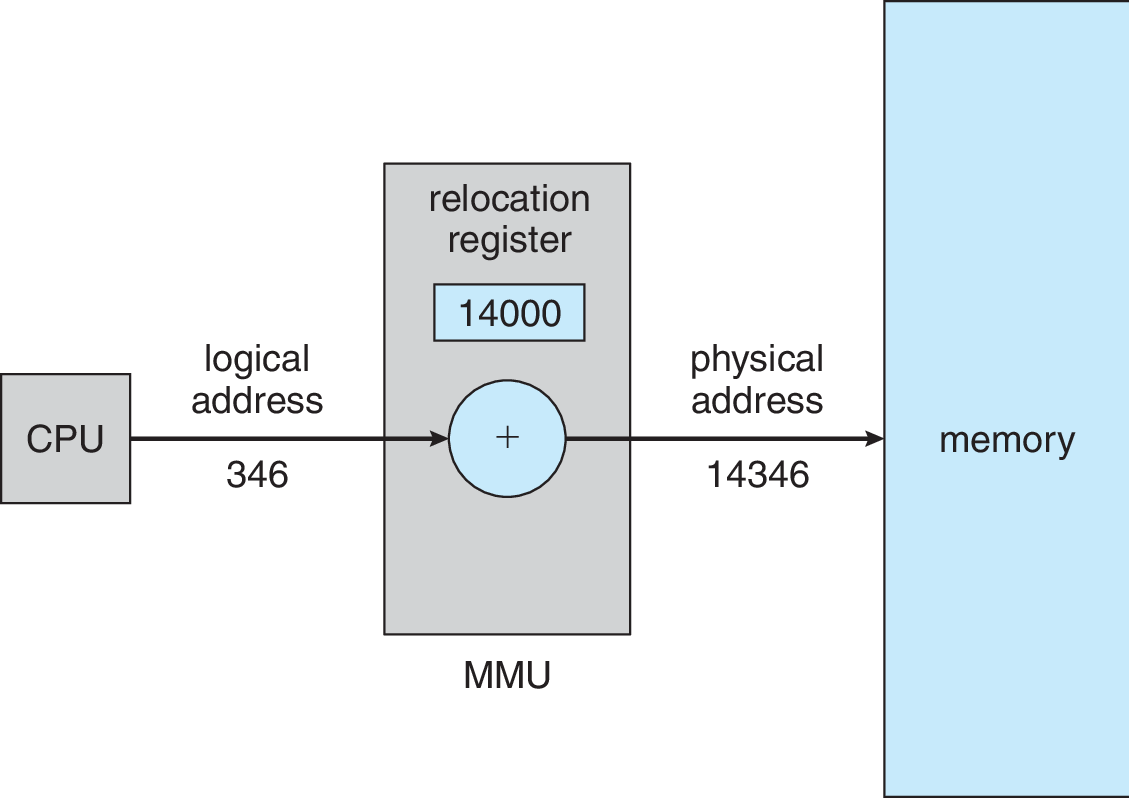
\includegraphics[width=5cm]{figs/02-8_04.pdf}
  \end{center}

\end{frame}


%---------------------------------------------------------------------
\begin{frame}
  \frametitle{Direccionamiento}
  \framesubtitle{Direcciones física y lógicas}

  Direccionamiento consiste en efectuar la transformación:
  \[
    f: \mathcal{L} \to \mathcal{F}
  \]
  $\mathcal{L}$: espacio de direcciones lógicas (o virtuales)

  $\mathcal{F}$: espacio de direcciones físicas

  \onslide<2->{Una versión muy simple.}
  
  \onslide<3->{Dado el registro de {\em relocation} $R$:
  \[
    f: \{0\ldots \mathit{max}\} \to \{R \ldots R + \mathit{max} \}
  \]
  \[
    f(d_L) = R + d_L
  \]
  }
  
\end{frame}
%---------------------------------------------------------------------
\begin{frame}
  \frametitle{Direccionamiento}
  \framesubtitle{Otros conceptos comunes}

  \begin{description}
    \item[{\bf Carga dinámica}] Cargar sólo parte del proceso. Cuando una rutina se necesita,
                                se carga la sección necesaria de código.
    \item[{\bf Bibliotecas}] Conjunto de rutinas de uso común que se {\em agregan} al programa
      \begin{itemize}
        \item {\bf Enlace Estático} ({\tt .lib}, {\tt .a}). Rutinas se enlazan dentro del binario final.
            \begin{itemize}
              \item +Rápido
              \item -Binario de mayor tamaño
              \item Modificación requiere re-compilación
            \end{itemize}
        \item {\bf Enlace Dinámico} ({\tt .dll}, {\tt .so}). Rutinas se enlazan con un {\em stub}: 
                              código representante de la rutina. Rutina se carga al llamarla.
            \begin{itemize}
              \item -Lento, pero sólo al primer acceso
              \item +Binario más pequeño
              \item Pueden reemplazarse {\em en caliente} (con un esquema de versiones)
            \end{itemize}
                              
      \end{itemize}
  \end{description}
  
\end{frame}

%---------------------------------------------------------------------
\begin{frame}
  \frametitle{{\em Swapping}}
%  \framesubtitle{Otros conceptos comunes}

  Traspaso {\em temporal} de memoria de un proceso a {\em memoria secundaria}
  
  \begin{center}
    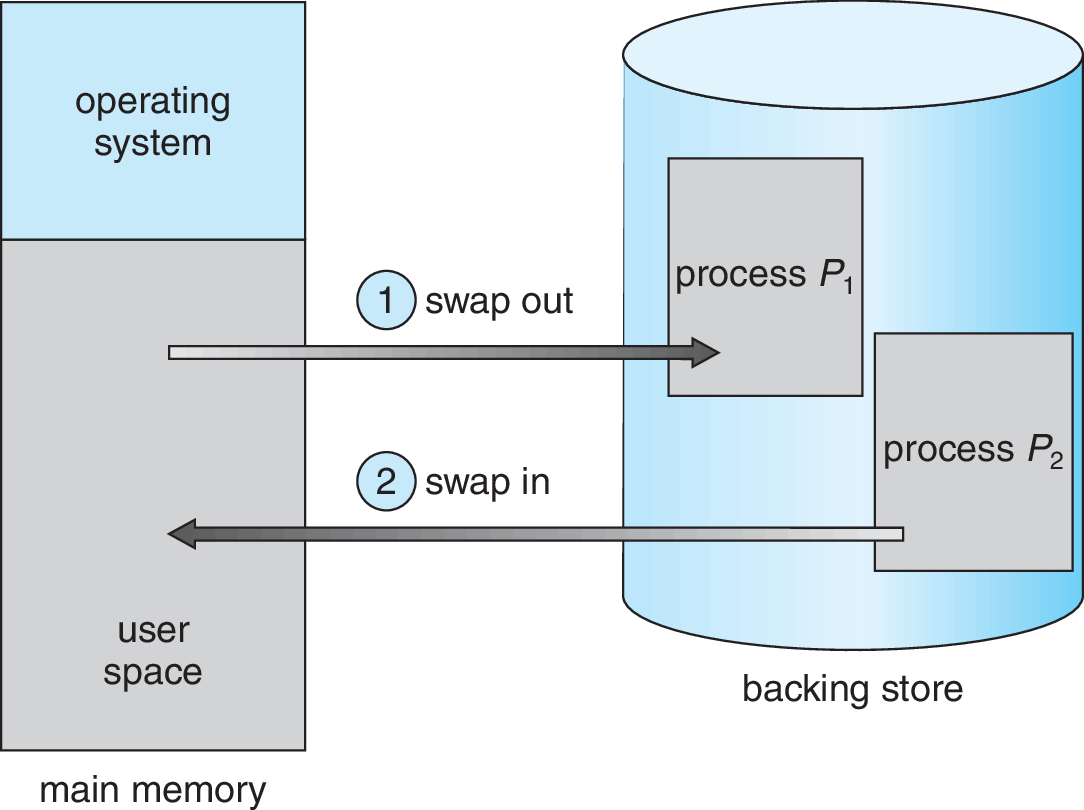
\includegraphics[width=5cm]{figs/02-8_05.pdf}
  \end{center}

  \begin{itemize}
    \item ¿Cuándo? Cuando queda poca memoria libre.
      \begin{itemize}
        \item Objetivo: maximizar el nivel de multiprogramación
      \end{itemize}
    \item ¿Cuánto? Todo, o lo que no esté utilizando
      \begin{itemize}
        \item Require informar al SO cuánta memoria se está utilizando
      \end{itemize}
    \item ¿Cuál? Uno que no esté en ejecución ni esperando E/S
      \begin{itemize}
        \item Pero pueden haber muchos criterios
      \end{itemize}
  \end{itemize}

\end{frame}

%---------------------------------------------------------------------
\subsection{Asignación contigua}

\begin{frame}
  \frametitle{Asignación contigua}
  \framesubtitle{La primera estrategia (adivinen si se usa)}

  Secciones bajas: Sistema Operativo
  
  A continuación se agrega cada proceso nuevo de manera contigua.
  
  \begin{itemize}
    \item MMU utiliza registro límite y registro de {\em relocation}
  \end{itemize}

  \begin{center}
    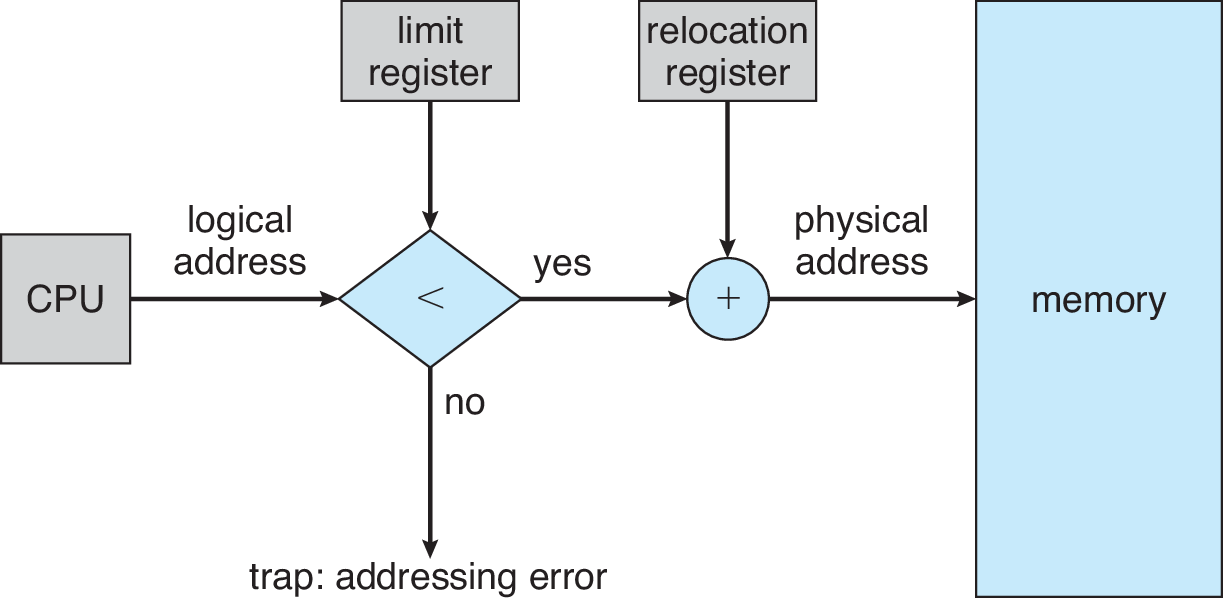
\includegraphics[width=8cm]{figs/02-8_06.pdf}
  \end{center}

  Procesos pueden ser {\em reubicados}
\end{frame}

%---------------------------------------------------------------------
%\begin{frame}
%  \frametitle{Asignación contigua}
%  \framesubtitle{¿Cómo dividir la memoria?}
%
%  Memoria se divide en {\em particiones}: una para cada proceso.
%  
%  El nivel de multiprogramación está dado por la cantidad de particiones.
%  
%  \begin{itemize}
%    \item Tamaño fijo: IBM OS/360
%    \item Tamaño variable: tabla indicando particiones ocupadas
%  \end{itemize}
%
%  \onslide<2->{Procesos se cargan en memoria solamente si hay espacios disponibles.}
%  
%  \onslide<3->{Cuando un proceso termina, su memoria es recuperada.}
%  
%
%\end{frame}
%---------------------------------------------------------------------
\begin{frame}
  \frametitle{Asignación contigua}
  \framesubtitle{¿Dónde ubicar el siguiente proceso?}

  Luego de algunas ejecuciones, el espacio queda con {\em huecos}.

  \onslide<2->{¿Dónde se carga el siguiente proceso?}
  
  \onslide<3->{Distintas estrategias de asignación:}
  \begin{itemize}
    \item<4->{\bf First-fit}. En el primer lugar disponible.
    \item<4->{\bf Best-fit}. En el que deja menos espacio libre (el más pequeño posible).
    \item<4->{\bf Worst-fit}. En el que deja más (el más grande).
  \end{itemize}
  
  \onslide<5->{¿Cuál es mejor?}
  \begin{itemize}
    \item <5-> Best-fit y First-fit suelen funcionar mejor que Worst-fit
    \item <5-> First-fit es más rápido
  \end{itemize}
\end{frame}

%---------------------------------------------------------------------
\begin{frame}
  \frametitle{Asignación contigua}
  \framesubtitle{Fragmentación}

  \begin{block}{{\bf Fragmentación externa}}
    \onslide<2->{Hay espacio para otro proceso, pero no contiguo.}
  \end{block}
    
  \begin{block}{{\bf Fragmentación interna}}
    \onslide<3->{Espacio sobre-asignado a procesos}

    \onslide<4->{Usualmente se asignan huecos en unidades de tamaño fijo}
  \end{block}

  \onslide<5->{¿Cómo evitar la fragmentación?}
    
\end{frame}
%---------------------------------------------------------------------
\begin{frame}
  \frametitle{Asignación contigua}
  \framesubtitle{Fragmentación}

  ¿Cómo evitar la fragmentación?
  
  \begin{itemize}
    \item<2-> Fusionando huecos: {\bf compactación}
      \begin{center}
        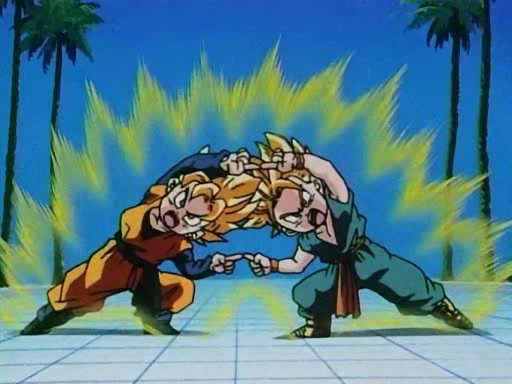
\includegraphics[width=3cm]{figs/02-fusion.png}
      \end{center}
      \begin{itemize}
		\item Requiere asignaciones en tiempo de ejecución
        \item Lento y costoso (en tiempo)
      \end{itemize}
    \item<3-> Mejor: realizar asignaciones {\bf no-contiguas}
      \begin{itemize}
        \item<4-> Después de todo, solo basta tener una buena transformación
        \item<4-> Dos técnicas: {\bf segmentación} y {\bf paginación}
      \end{itemize}
  \end{itemize}

\end{frame}
%---------------------------------------------------------------------
\subsection{Segmentación}

\begin{frame}
  \frametitle{Segmentación}
  
  La ``visión del programador'' de su propio código no es necesariamente la misma
  que ocurre en la memoria física.
  
  Programador suele pensar en:
  \begin{itemize}
    \item Funciones y métodos
    \item Memoria de {\em Heap}
    \item {\em Stack} de ejecución
    \item Bibliotecas
    \item Variables y objetos
  \end{itemize}
  
  Memoria sólo ve una secuencia de bytes
  
  \begin{block}{Idea de la Segmentación}
    En lugar de asignar memoria contiguamente, se asigna memoria a {\em segmentos} del programa.
  \end{block}
\end{frame}

%---------------------------------------------------------------------
\begin{frame}
  \frametitle{Segmentos de un programa en C}

  \begin{columns}[c]
    \begin{column}[T]{7cm}
      Un compilador de C típicamente genera segmentos para:
      \begin{itemize}
        \item Código
        \item Variables globales
        \item {\em Heap} (para asignación dinámica de memoria)
        \item {\em Stacks} para cada {\em thread}
        \item Código de la librería estándar de C
      \end{itemize}
    \end{column}
    
    \begin{column}[T]{4cm}
      \begin{center}
        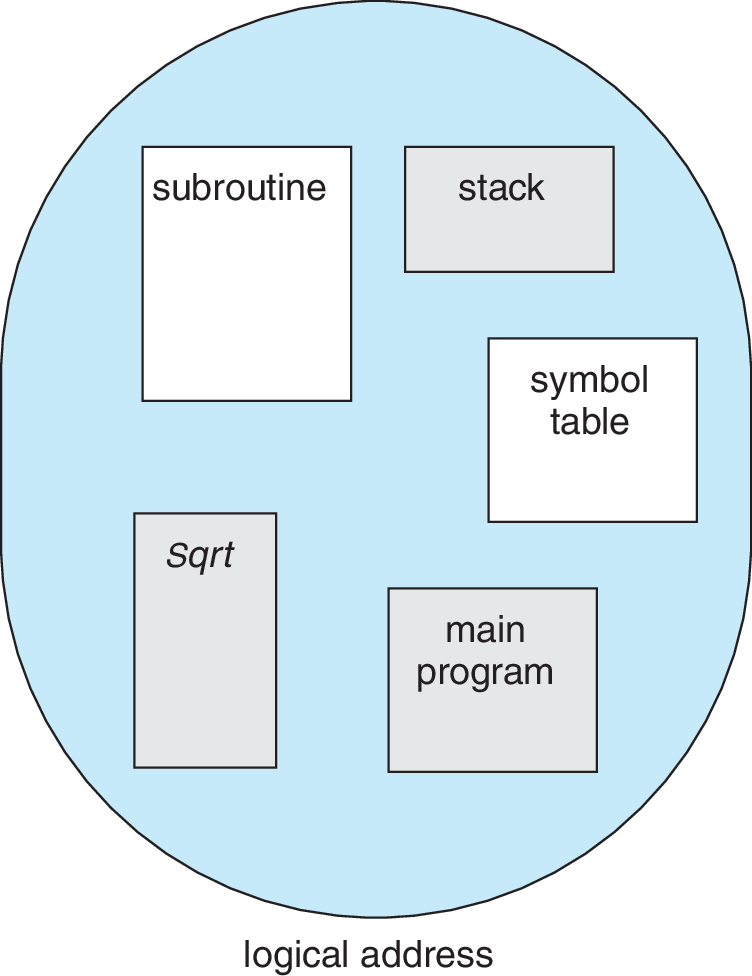
\includegraphics[width=4cm]{figs/02-8_07.pdf}
      \end{center}
    \end{column}
  \end{columns}
  
\end{frame}

%---------------------------------------------------------------------
\begin{frame}
  \frametitle{¿Segmentos?}

  Segmentos tienen:
  \begin{itemize}
    \item Nombre (identificador)
    \item Longitud
  \end{itemize}

  Una dirección de memoria específica en memoria segmentada está formada por una tupla con dos datos (un par):
  \begin{center}
  $\langle$ {\tt numeroDeSegmento}, {\tt offset} $\rangle$
  \end{center}
  
  {\bf Sin embargo,} la dirección de memoria es {\em unidimensional}.
  ¿Cómo indicar ambos valores?
\end{frame}


%---------------------------------------------------------------------
\begin{frame}
  \frametitle{MMU para segmentación}

    \begin{itemize}
      \item Dirección lógica es $\langle$ segmento, offset $\rangle$
      \item Asociación se hace con una {\bf tabla de segmentos} con valores {\bf base} y {\bf límite}
    \end{itemize}

    \begin{center}
      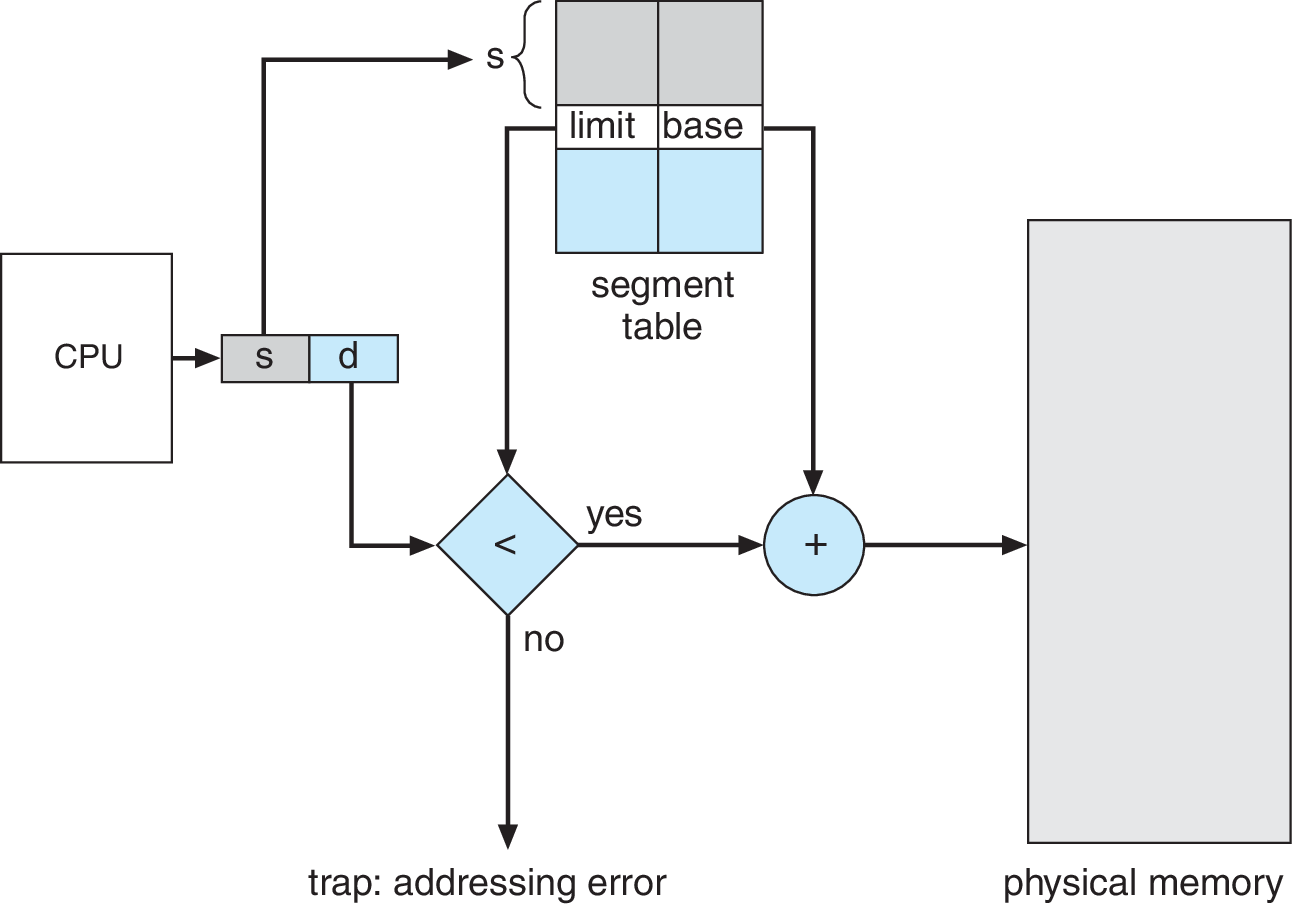
\includegraphics[width=8cm]{figs/02-8_08.pdf}
    \end{center}

\end{frame}

%---------------------------------------------------------------------
\begin{frame}
  \frametitle{Ejemplo de Segmentación}

  \begin{center}
    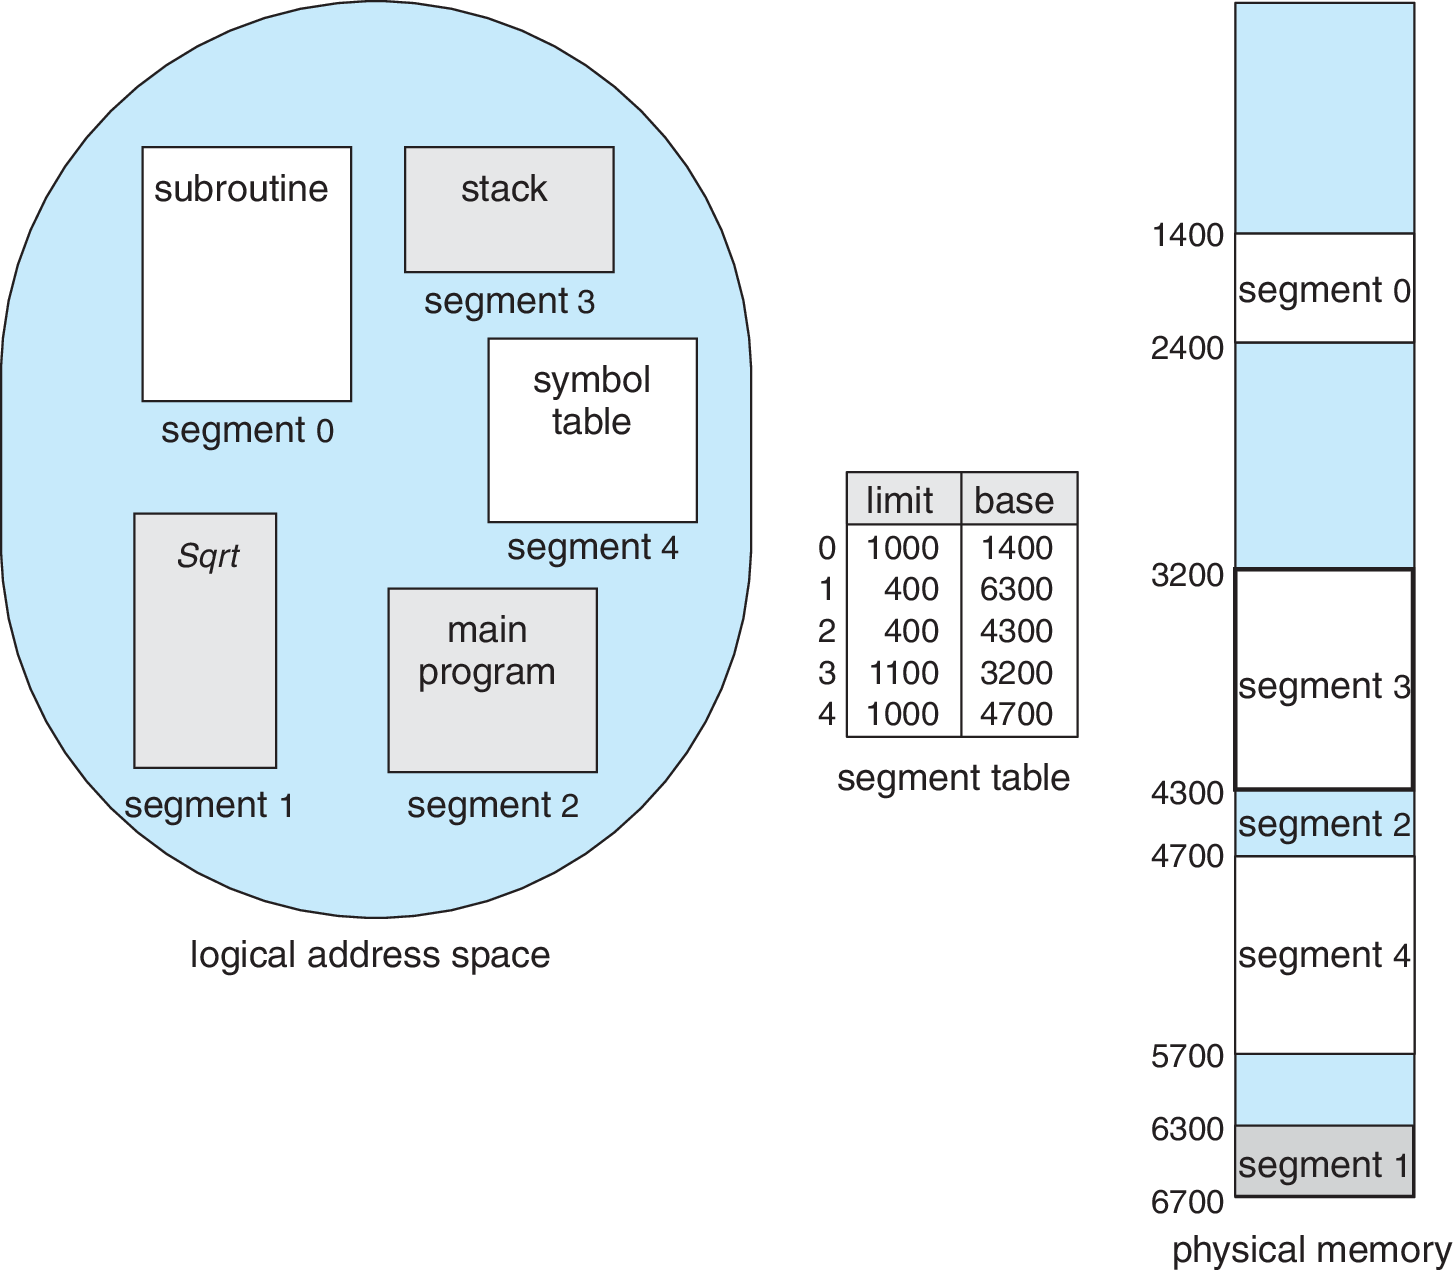
\includegraphics[width=8cm]{figs/02-8_09.pdf}
  \end{center}


\end{frame}
%---------------------------------------------------------------------
\begin{frame}
  \frametitle{Límites de la Segmentación}

  \begin{itemize}
    \item Permite asignar porciones de memoria del proceso a distintos
          sectores de memoria física.
    \item Asignación de segmentos aún es contigua.
    \item Problema se ha reducido de tamaños de memoria ``grandes'' a tamaños
          pequeños.
  \end{itemize}
  {\bf Aún puede haber fragmentación externa}
\end{frame}

%---------------------------------------------------------------------
\subsection{Paginación}

\begin{frame}
  \frametitle{Paginación}

  Dos divisiones en unidades de tamaño fijo:
  \begin{itemize}
    \item Memoria física se divide en {\bf frames} (marcos)
    \item Memoria lógica se divide en {\bf páginas}
  \end{itemize}
  
  Memoria se carga en trozos de tamaño fijo
  
  \begin{itemize}
    \item Permite separar el espacio de direcciones lógico ($\mathcal{L}$) del espacio de direcciones físico ($\mathcal{F}$).
    \item Permite que $|\mathcal{L}| > |\mathcal{F}|$
      \begin{itemize}
        \item No es menor. Sistema con $2^{32}$ (4G) direcciones de memoria física
              puede albergar procesos con direcciones de 64-bit.
      \end{itemize}
  \end{itemize}
  
\end{frame}

%---------------------------------------------------------------------
\begin{frame}
  \frametitle{Paginación}

  Dirección de memoria paginada contiene:
  \begin{center}
    $\langle$ {\tt numeroDePagina}, {\tt offset} $\rangle$
  \end{center}

  \begin{center}
    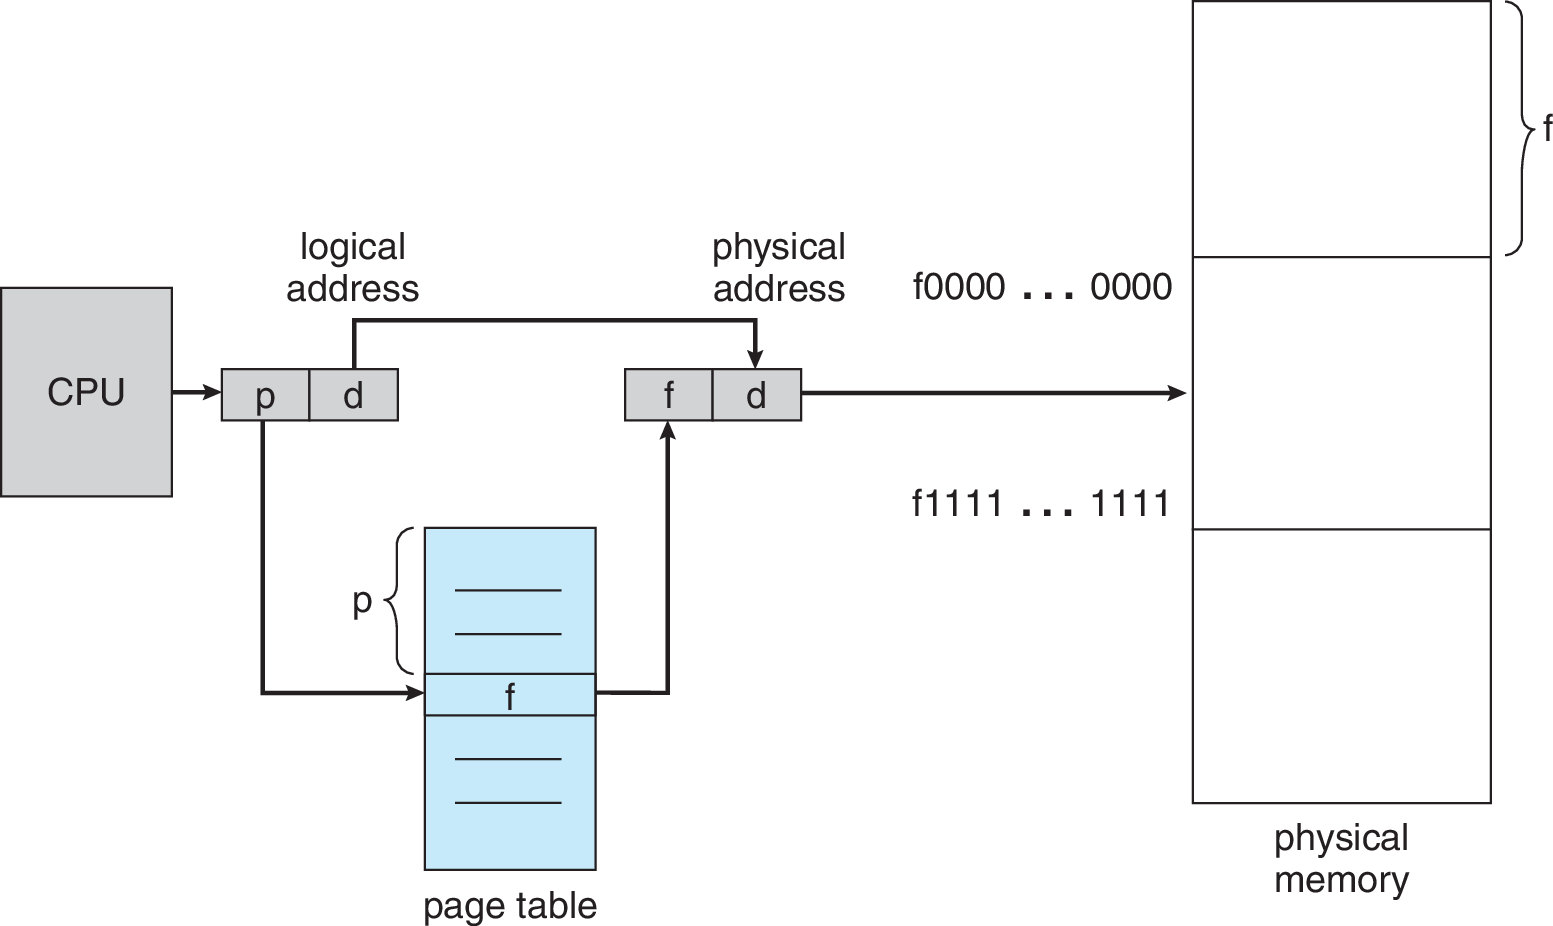
\includegraphics[width=9cm]{figs/02-8_10.pdf}
  \end{center}


\end{frame} 
%---------------------------------------------------------------------
\begin{frame}
  \frametitle{Ejemplo de Paginación}

  \begin{center}
    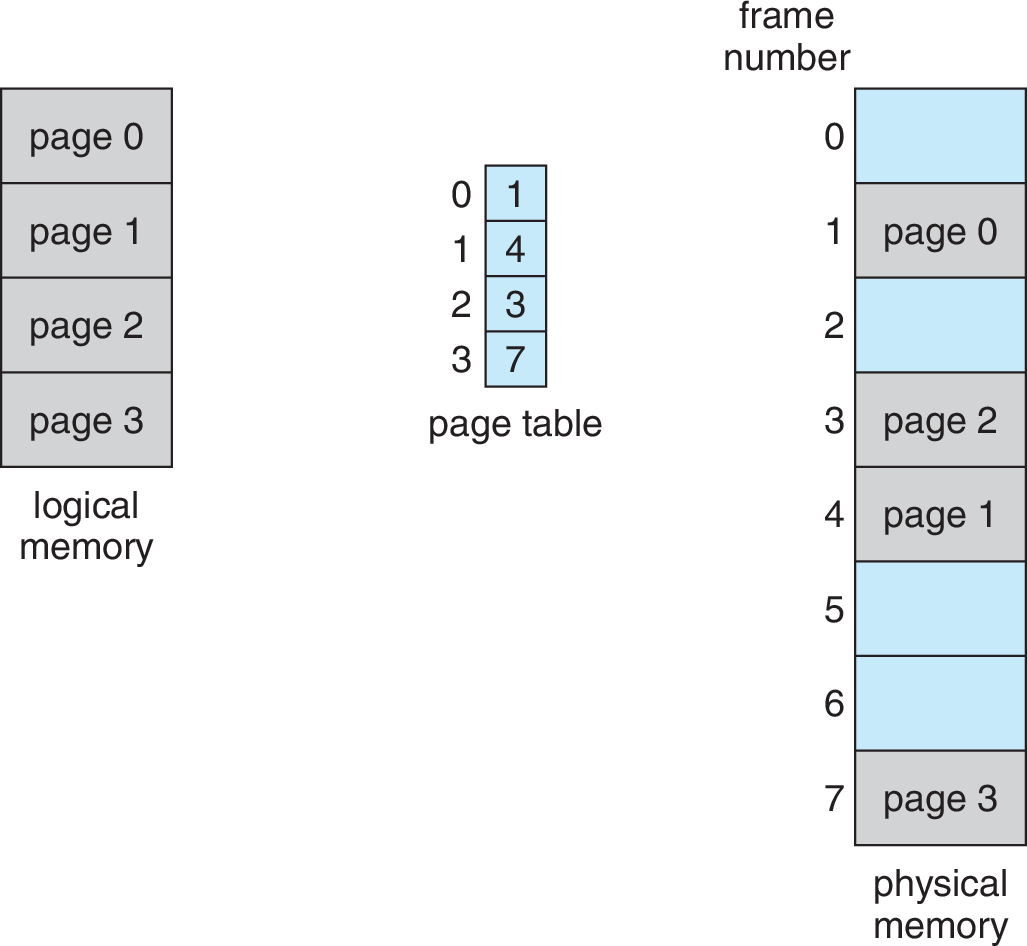
\includegraphics[width=8cm]{figs/02-8_11.pdf}
  \end{center}
  

\end{frame}
%---------------------------------------------------------------------
\begin{frame}
  \frametitle{Tamaños de páginas y frames}

  \begin{itemize}
    \item Tamaño de páginas y frames determinado por {\em hardware}
    \item Típicamente potencia de 2. Entre 512 bytes a 1GB por página.
    \item ¿Por qué potencia de 2? \ldots Hace todo más fácil
      \begin{itemize}
        \item Transformación se hace reemplazando bits de la dirección lógica
        \item No requiere operaciones adicionales
      \end{itemize}
  \end{itemize}
  Ejemplo:
  \begin{itemize}
    \item Direcciones lógicas de $m$-bit
    \item Tamaño de página de $2^n$ bytes
      \begin{center}
        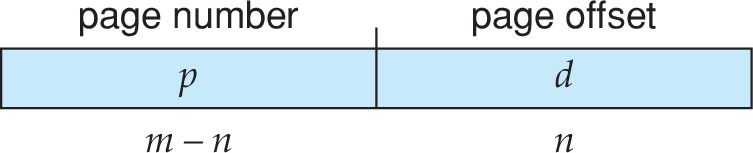
\includegraphics[width=7cm]{figs/02-in-8_1.pdf}
      \end{center}
  \end{itemize}
  
\end{frame}
%---------------------------------------------------------------------
\begin{frame}
  \frametitle{Ejemplo de paginación}

  Páginas de $2^n$ bytes, $n=2$. Direcciones lógicas de $m$-bit, $m=4$.
  
  Memoria física de 32 bytes == 8 páginas.
  
  \begin{center}
    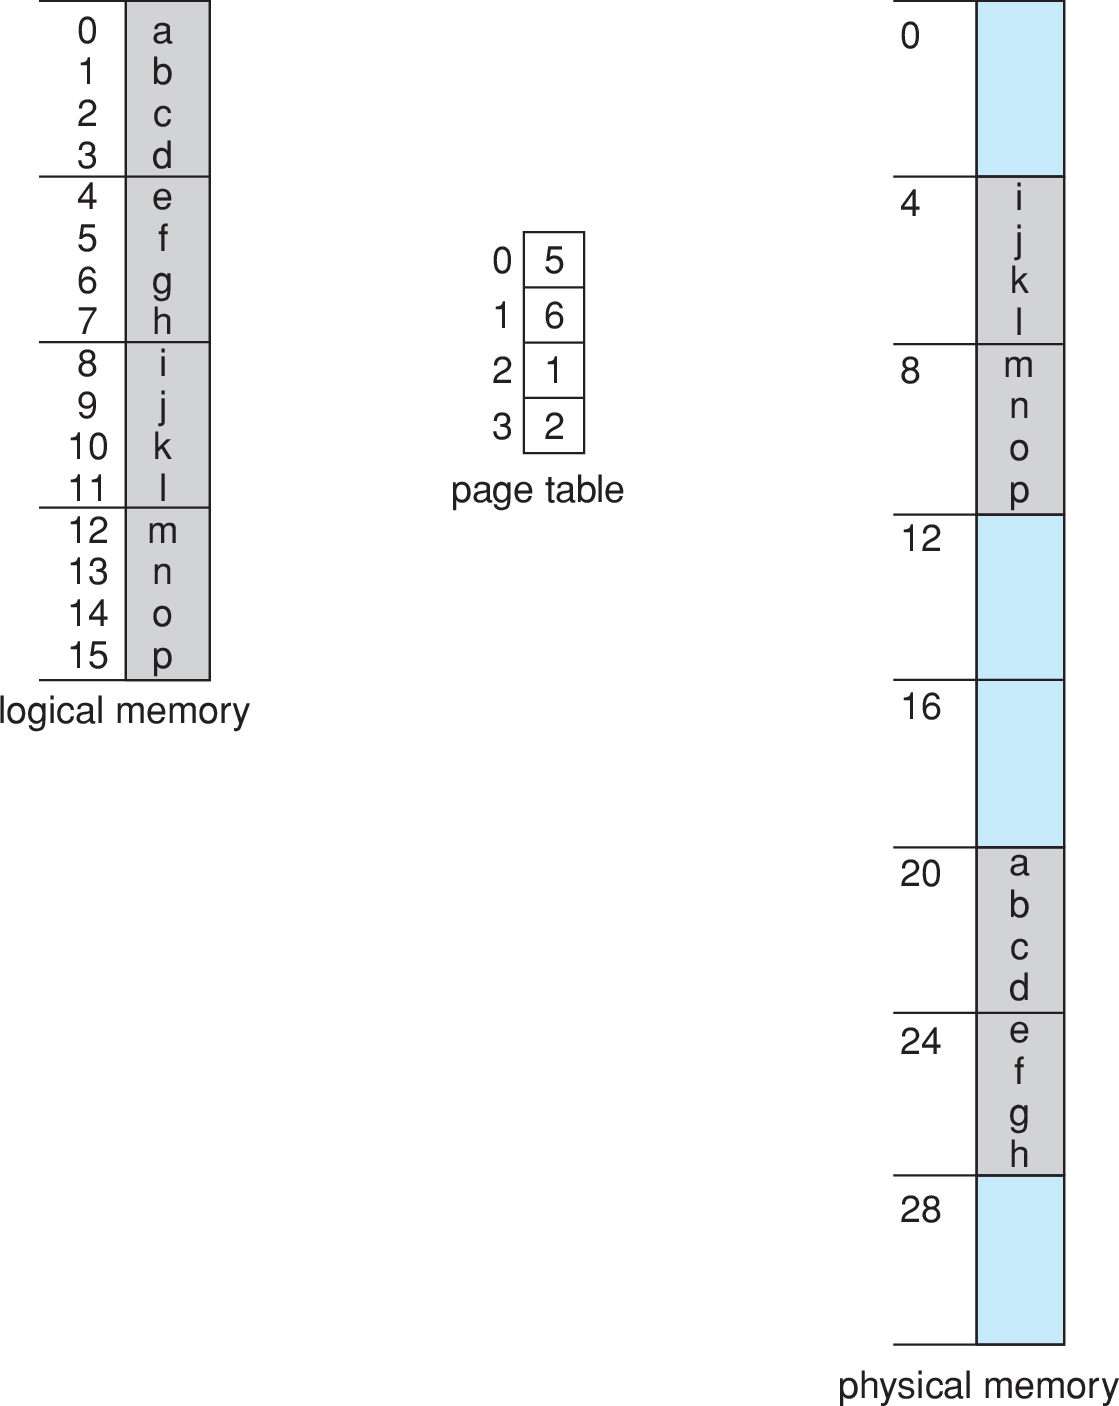
\includegraphics[width=5.2cm]{figs/02-8_12.pdf}
  \end{center}

\end{frame}
%---------------------------------------------------------------------
\begin{frame}
  \frametitle{Límites de la paginación}

  \begin{itemize}
    \item ¿Fragmentación externa? \onslide<2->{\ldots ¡0!}
    \item<2-> Se produce fragmentación interna
      \begin{itemize}
        \item Páginas de 4KB.
        \item<3-> Si el proceso necesita $20\times 4\text{KB} + 512\text{B}$,
              se asignan 21 páginas.
        \item<4-> Se pierden $4096 - 512 = 3584$ bytes
        \item<5-> Peor caso: solicitud de $N$ páginas más $1$ byte 
                  asigna $N+1$ páginas.
      \end{itemize}
  \end{itemize}
  
\end{frame}

%---------------------------------------------------------------------
\begin{frame}
  \frametitle{Tamaño de la tabla de páginas}

  Ejemplo: DEC PDP-11. Máquina de 16-bit, $1970\sim 1990$

  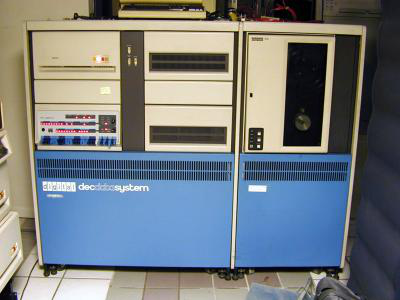
\includegraphics[width=5cm]{figs/02-PDP-11-70-DDS570.png}
  \hfill
  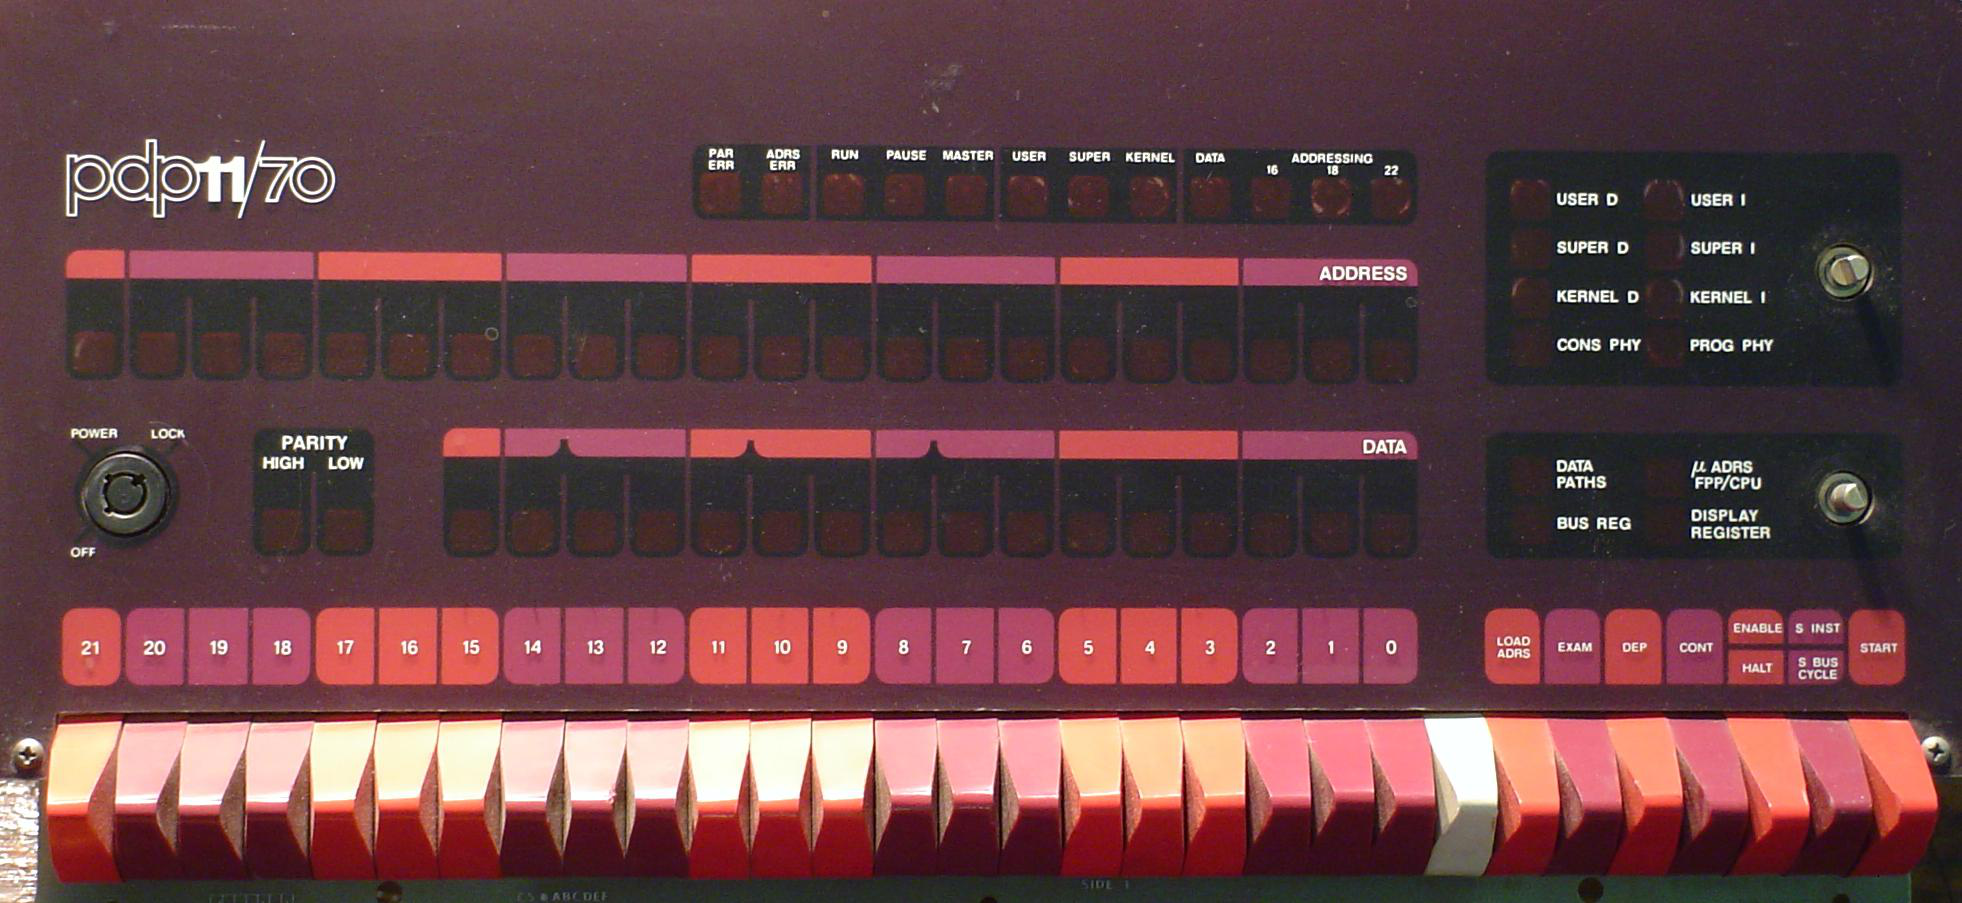
\includegraphics[width=5cm]{figs/02-Pdp-11-70-panel.png}
  
  Páginas de 8KB. ¿Tamaño de la tabla de páginas?
  
\end{frame}

%---------------------------------------------------------------------
\begin{frame}
  \frametitle{Tamaño de la tabla de páginas}

  Otro ejemplo: 32-bit. Páginas de 4KB.

  ¿Tamaño de la tabla de páginas?  
  \onslide<2->{¡$2^{20}$ entradas!}
  \begin{itemize}
    \item <3->{Accesos pueden hacerse lentos}
    \item <4->{¿Solución? Otro tipo de {\em caché}}
  \end{itemize}
  
  \onslide<5->{
  {\bf Translation Look-aside Buffer} (TLB)
  \begin{itemize}
    \item Subconjunto de tabla de páginas en registro de rápido acceso
    \item Entre 32 a 1024 entradas
  \end{itemize}
  }

\end{frame}
%---------------------------------------------------------------------
\begin{frame}
  \frametitle{{\em Translation Look-aside Buffer}}

  \begin{center}
    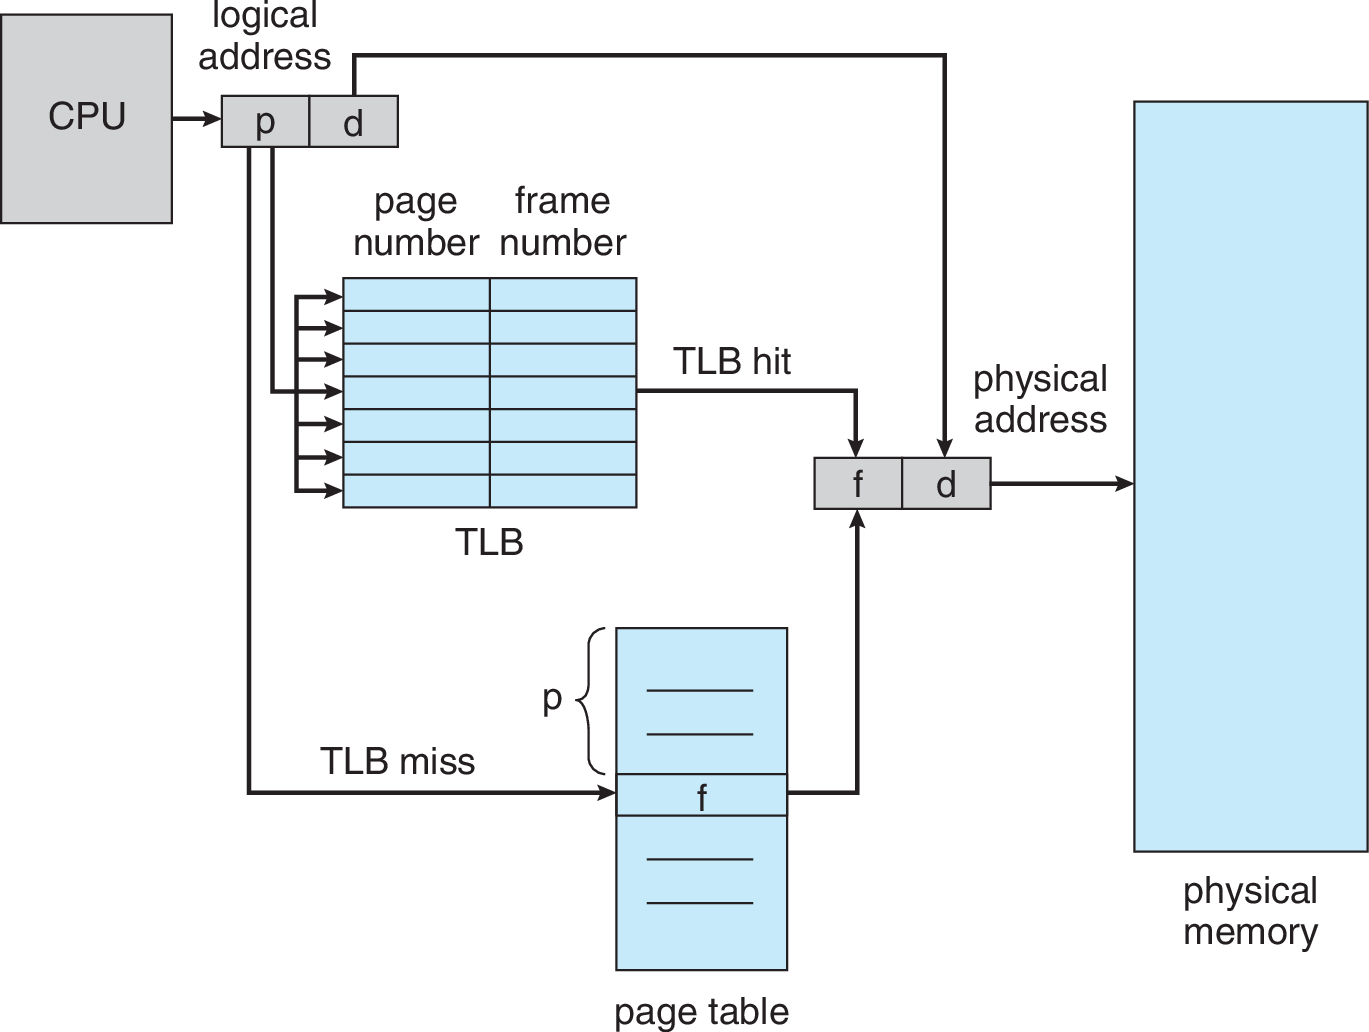
\includegraphics[width=9cm]{figs/02-8_14.pdf}
  \end{center}

\end{frame}

%---------------------------------------------------------------------
\subsection{Tablas de Páginas}

\begin{frame}
  \frametitle{Tablas de Páginas}

  Tablas de páginas pueden implementarse de distintas maneras
  
  \onslide<2->{Tamaños comunes:}
  \begin{itemize}
    \item<3-> Direcciones lógicas de 32-bit. \onslide<4->{$2^{32}=4G$ direcciones}
    \item<5-> Páginas de $4\text{KB}=2^{12}$
    \item<6-> Tabla puede tener hasta $2^{20}$ entradas. 
    \item<7-> Si cada entrada ocupa 4 bytes, la tabla de páginas ocupa $4\text{MB}$
    \item<8-> ¡La tabla de páginas no cabe en una página!
  \end{itemize}
\end{frame}

%---------------------------------------------------------------------
\begin{frame}
  \frametitle{Tablas de Páginas Jerárquicas}

  Ejemplo: esquema de dos niveles

  \begin{center}
    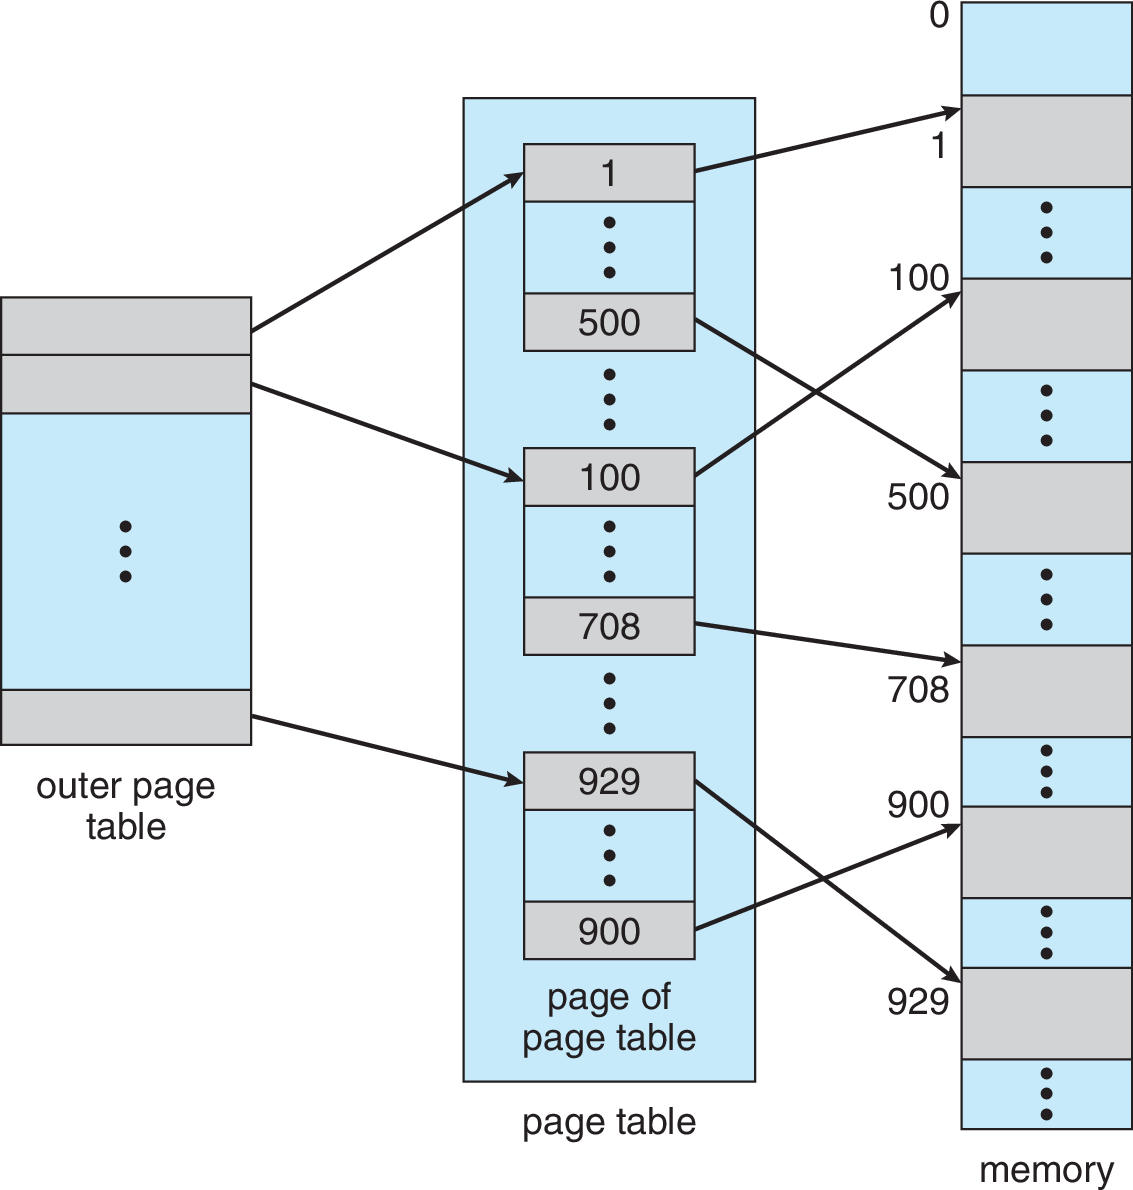
\includegraphics[width=6cm]{figs/02-8_17.pdf}
  \end{center}
  
  
\end{frame}
%---------------------------------------------------------------------
\begin{frame}
  \frametitle{Tablas de Páginas Jerárquicas}

  Direccionamiento de dos niveles

  \begin{center}
    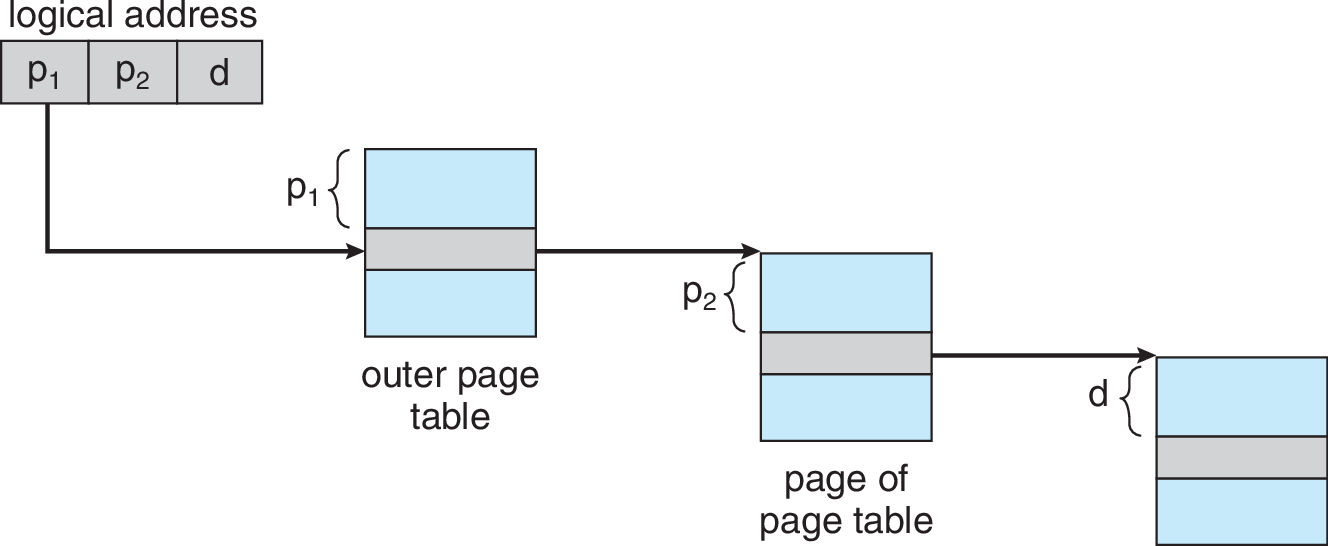
\includegraphics[width=9cm]{figs/02-8_18.pdf}
  \end{center}
  
  \begin{center}
    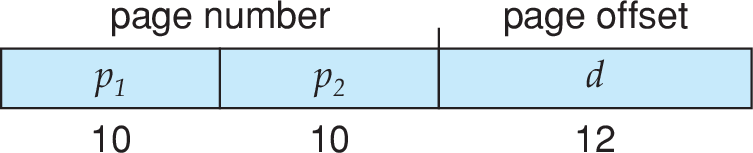
\includegraphics[width=6cm]{figs/02-in-8_2.pdf}
  \end{center}
  

\end{frame}

%---------------------------------------------------------------------
\begin{frame}
  \frametitle{Tablas de Páginas Jerárquicas}

  ¿Cuántos niveles? 
  
  Ejemplo: Direcciones de 64-bit

  \begin{center}
    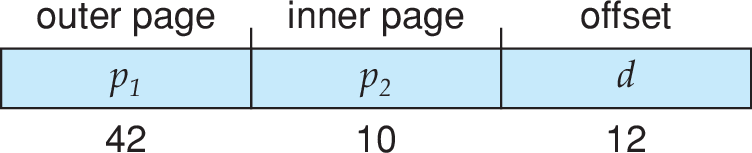
\includegraphics[width=6cm]{figs/02-in-8_4.pdf}
  \end{center}

  \onslide<2->{Otro nivel de paginación \ldots}
  
  \onslide<3->{
  \begin{center}
    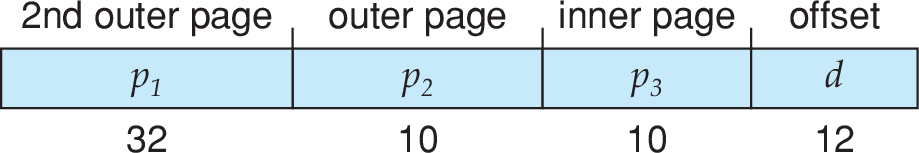
\includegraphics[width=6cm]{figs/02-in-8_5.pdf}
  \end{center}  
  }

  \onslide<4->{64-bit UltraSPARC poseía 7 niveles de paginación}
  
\end{frame}

%---------------------------------------------------------------------
\begin{frame}
  \frametitle{Tablas de Páginas con {\em hash}}

  \begin{center}
    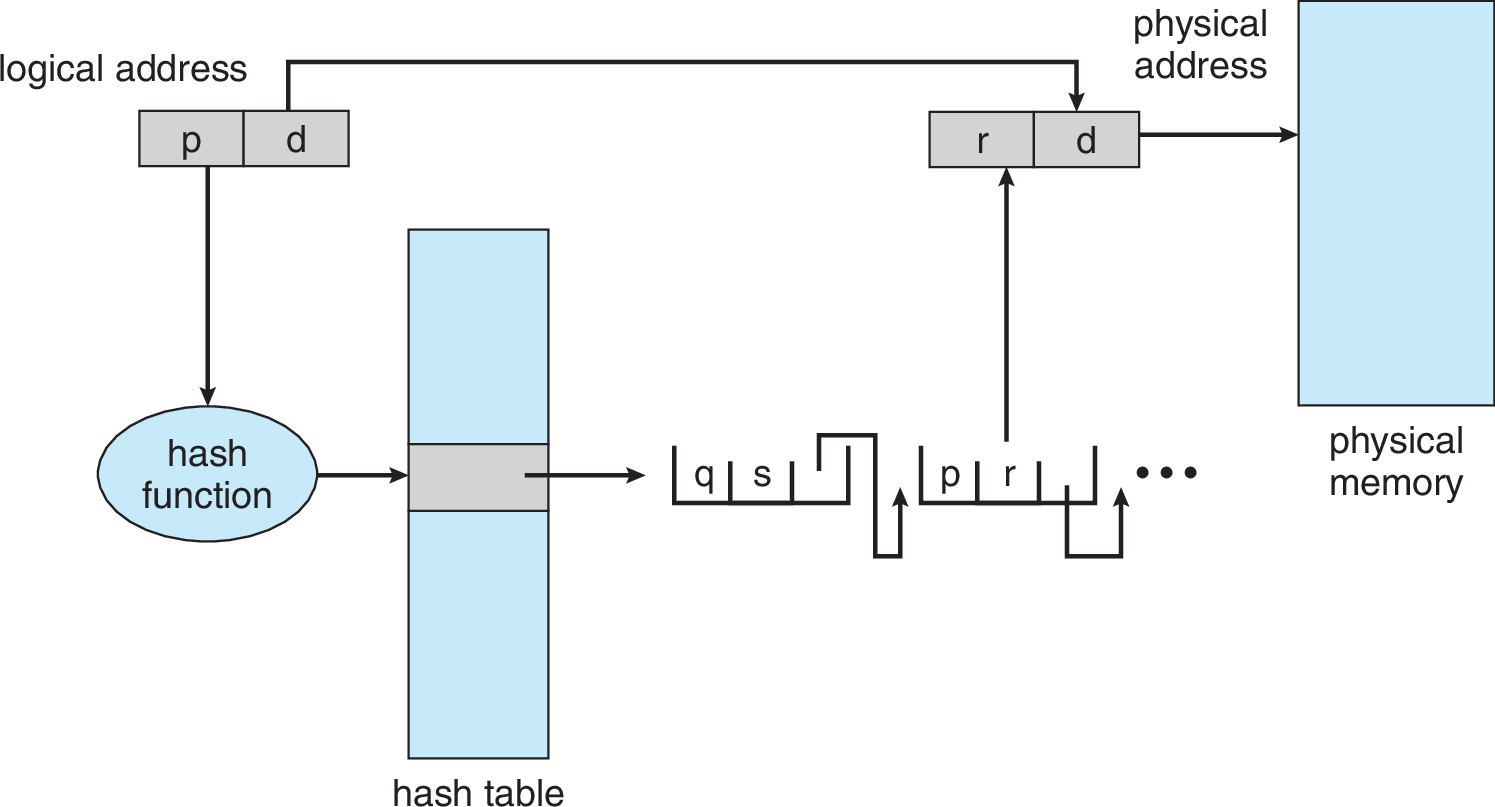
\includegraphics[width=9cm]{figs/02-8_19.pdf}
  \end{center}

  Apropiadas para espacios de direcciones {\em sparse} (ralos)

\end{frame}

%---------------------------------------------------------------------
\begin{frame}
  \frametitle{Tablas de Páginas invertidas}

  \begin{itemize}
    \item Una entrada por frame (en lugar de página)
    \item Sólo una tabla en el sistema (no por proceso)
  \end{itemize}

  \begin{center}
    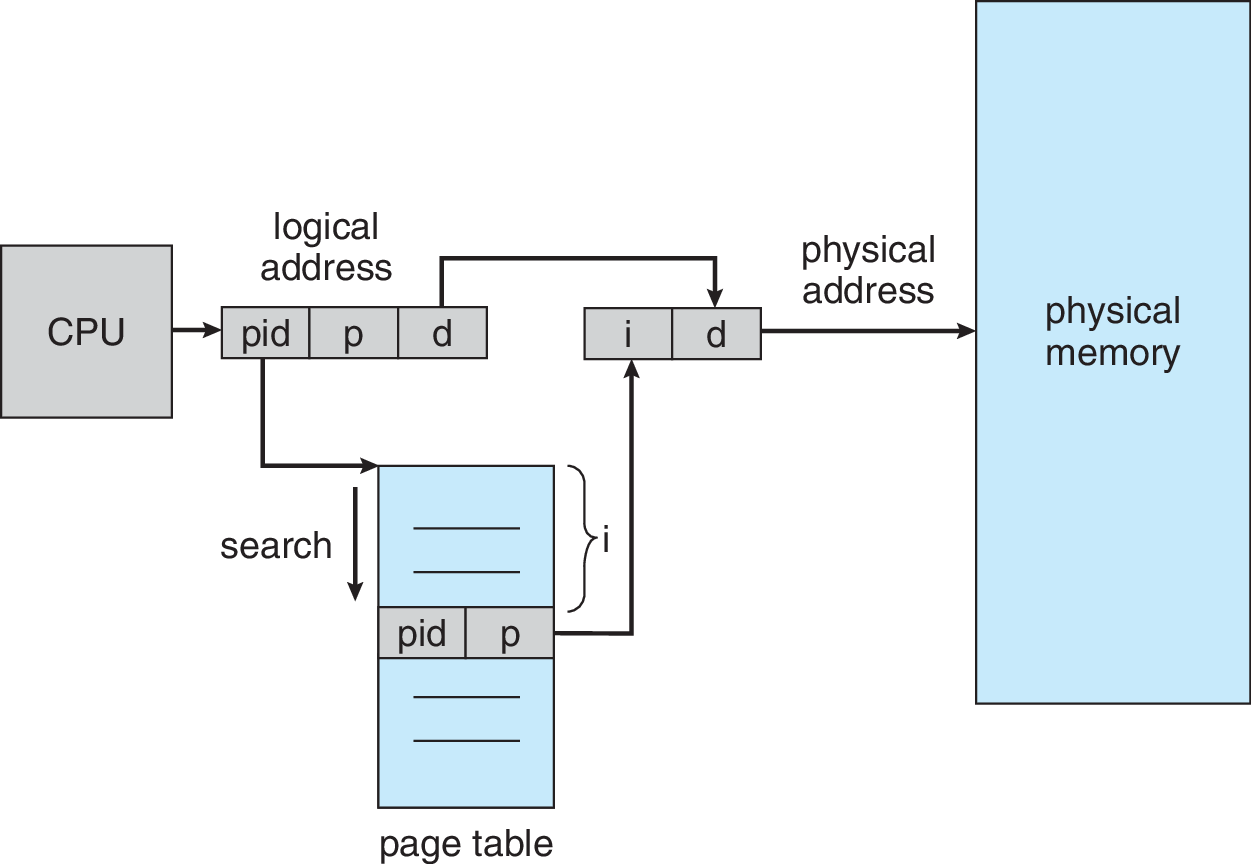
\includegraphics[width=8cm]{figs/02-8_20.pdf}
  \end{center}

  Usada en 64-bit UltraSPARC, y PowerPC

\end{frame}
%---------------------------------------------------------------------
\section{Memoria Virtual}

\subsection{Funcionamiento}

\begin{frame}
  \frametitle{Funcionamiento}

  Estrategias de direccionamiento
  
  \begin{itemize}
    \item Orientadas a dar ilusión de que todo el programa se encuentra en memoria contínua
    \item Pero \ldots aún se necesita al programa completo cargado en memoria
    \item ¿Y la carga dinámica?
      \begin{itemize}
        \item Hace la carga más rápida, pero una vez cargado debe seguir en memoria
        \item A menos que se haga {\em swap}
      \end{itemize}
  \end{itemize}

  \onslide<2->{
  Pero mantener todo el programa en memoria es muy restrictivo
  }
  \begin{itemize}
    \item<3-> No todas las partes del código se requieren simultáneamente
    \item<3-> Un proceso que solicita más memoria que la memoria física disponible no podría cargarse
  \end{itemize}
\end{frame}

%---------------------------------------------------------------------
\begin{frame}
  \frametitle{Funcionamiento}

  {\bf Memoria Virtual} aumenta la separación entre la memoria visible por el programador,
  y la memoria física de la máquina en que se ejecuta el programa.
  
  \begin{center}
    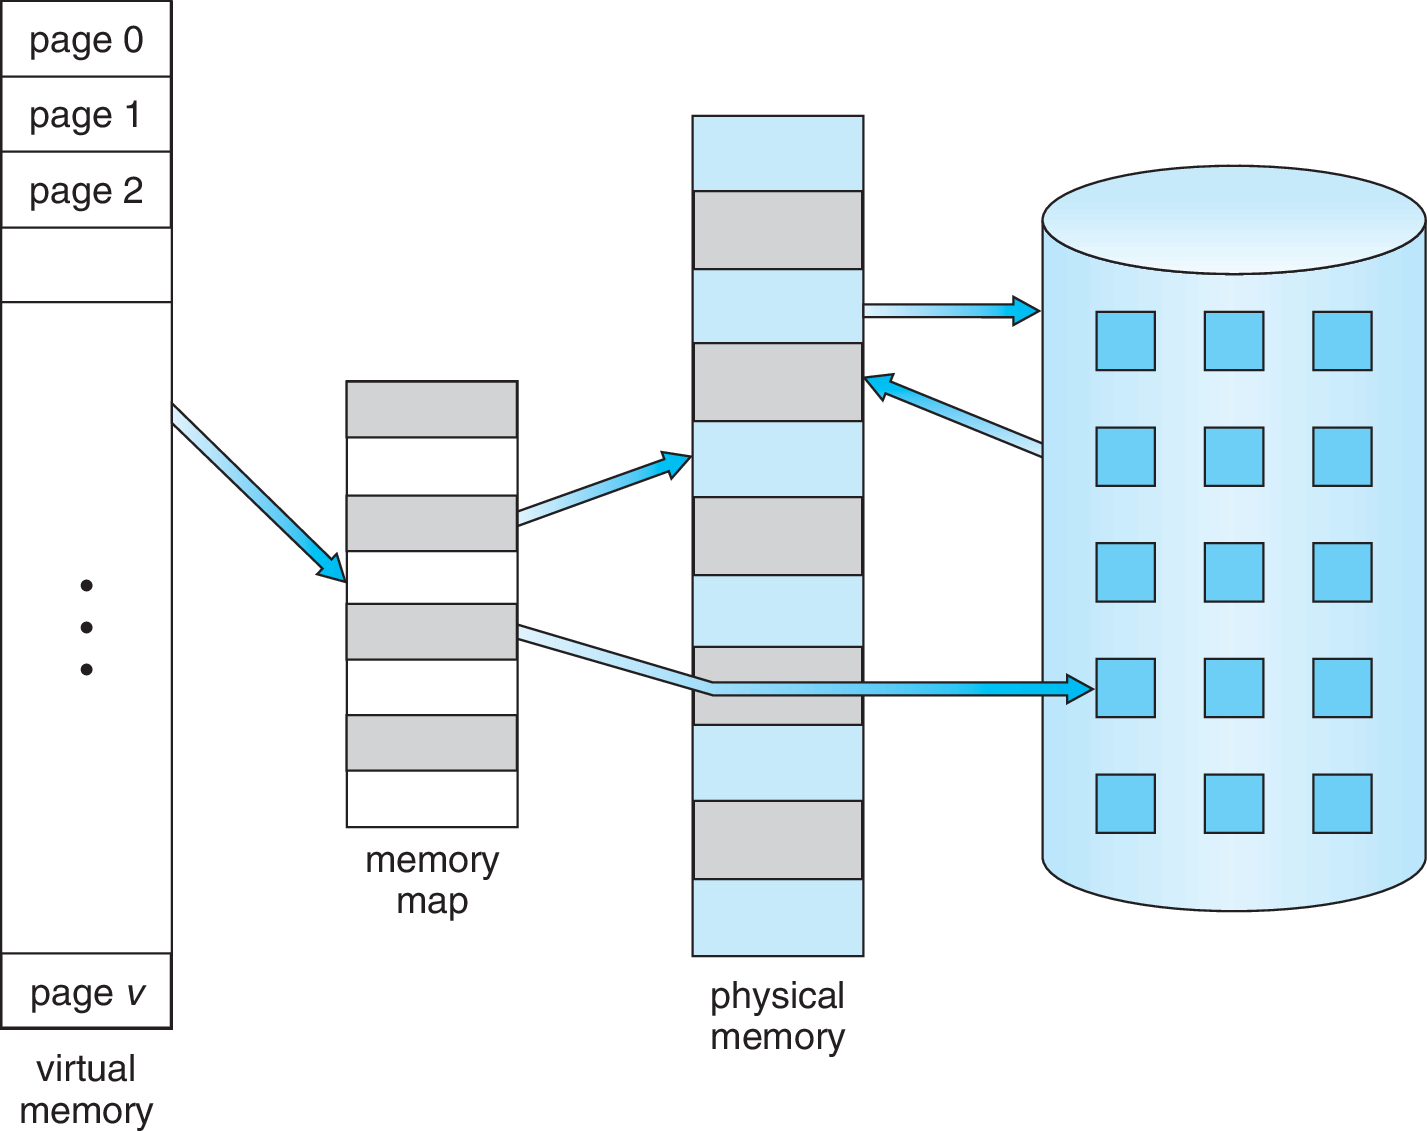
\includegraphics[width=8cm]{figs/02-9_01.pdf}
  \end{center}


\end{frame}
%---------------------------------------------------------------------
%\begin{frame}
%  \frametitle{Funcionamiento}
%
%  Bibliotecas compartidas se asigna a {\em frames} ya cargados
%  
%  \begin{center}
%    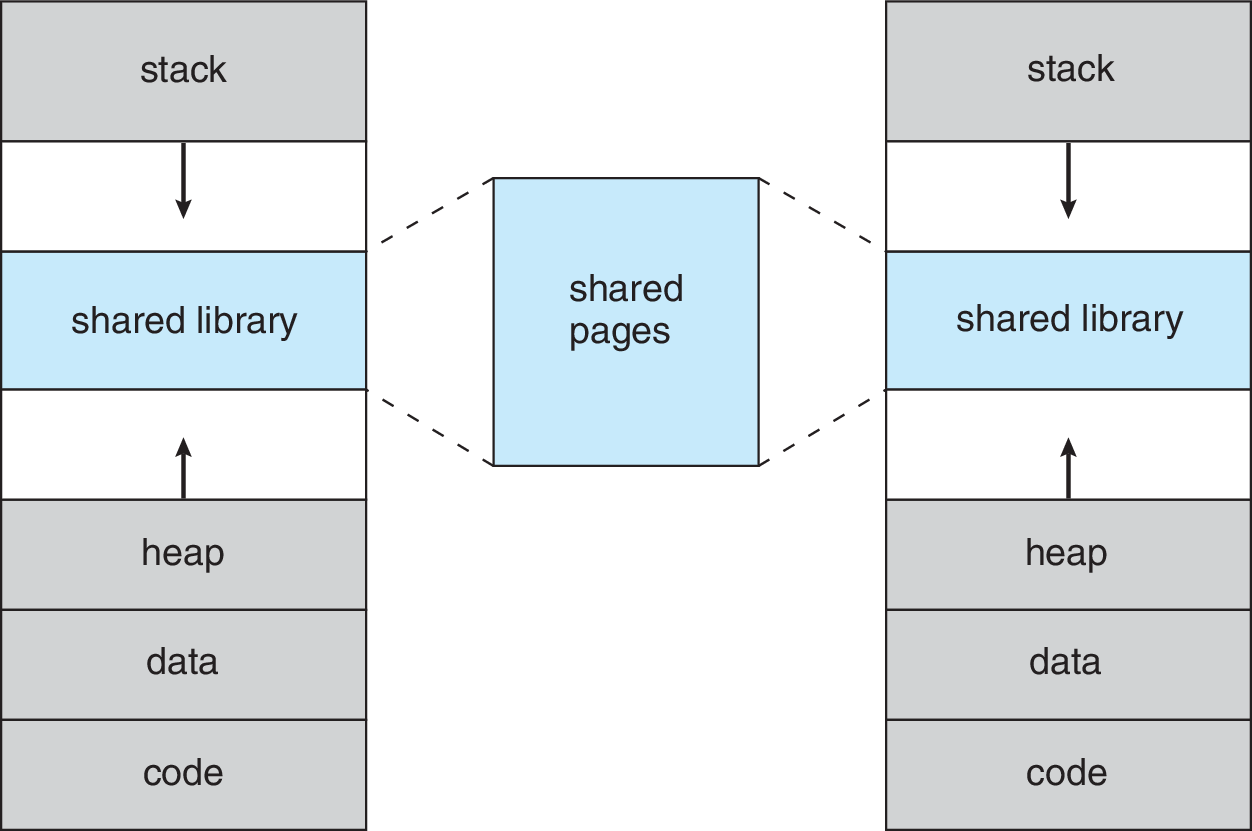
\includegraphics[width=8cm]{figs/02-9_03.pdf}
%  \end{center}
%
%\end{frame}
%---------------------------------------------------------------------
\subsection{Paginación por demanda}

\begin{frame}
  \frametitle{Paginación por demanda}

  Primera etapa: mantener registro de páginas cargadas
  \begin{itemize}
    \item Bit adicional en tabla de páginas
      \begin{itemize}
        \item {\em Valid}: Página en memoria
        \item {\em Invalid}: Página almacenada en disco, pero no en memoria
      \end{itemize}
    \item Al detectar un acceso a una página {\em inválida}, ésta se carga dinámicamente
          y se establece el bit a {\em valid}
  \end{itemize}

  \begin{center}
    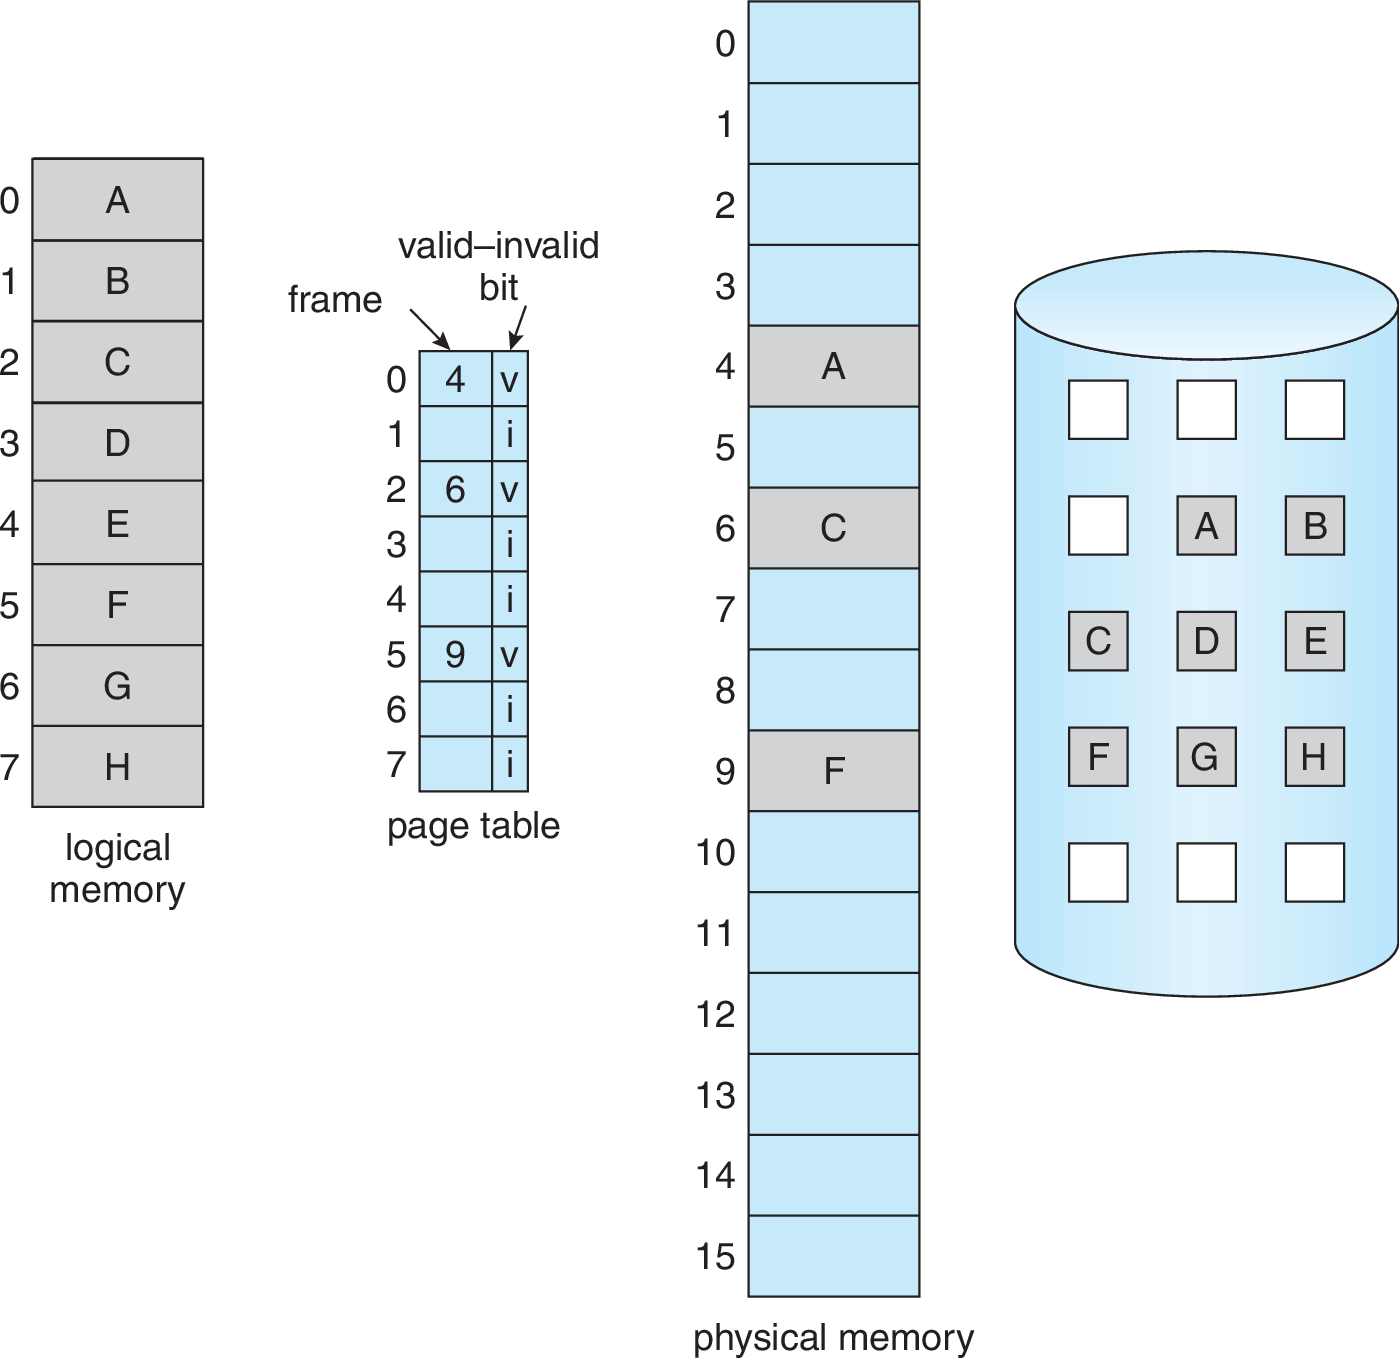
\includegraphics[width=5cm]{figs/02-9_05.pdf}
  \end{center}
  
\end{frame}

%---------------------------------------------------------------------
\begin{frame}
  \frametitle{Paginación por demanda}

  Segunda etapa: cargar páginas que se necesiten
  
  \begin{itemize}
    \item Proceso de carga se activa ante un {\bf page-fault}
  \end{itemize}

  \begin{center}
    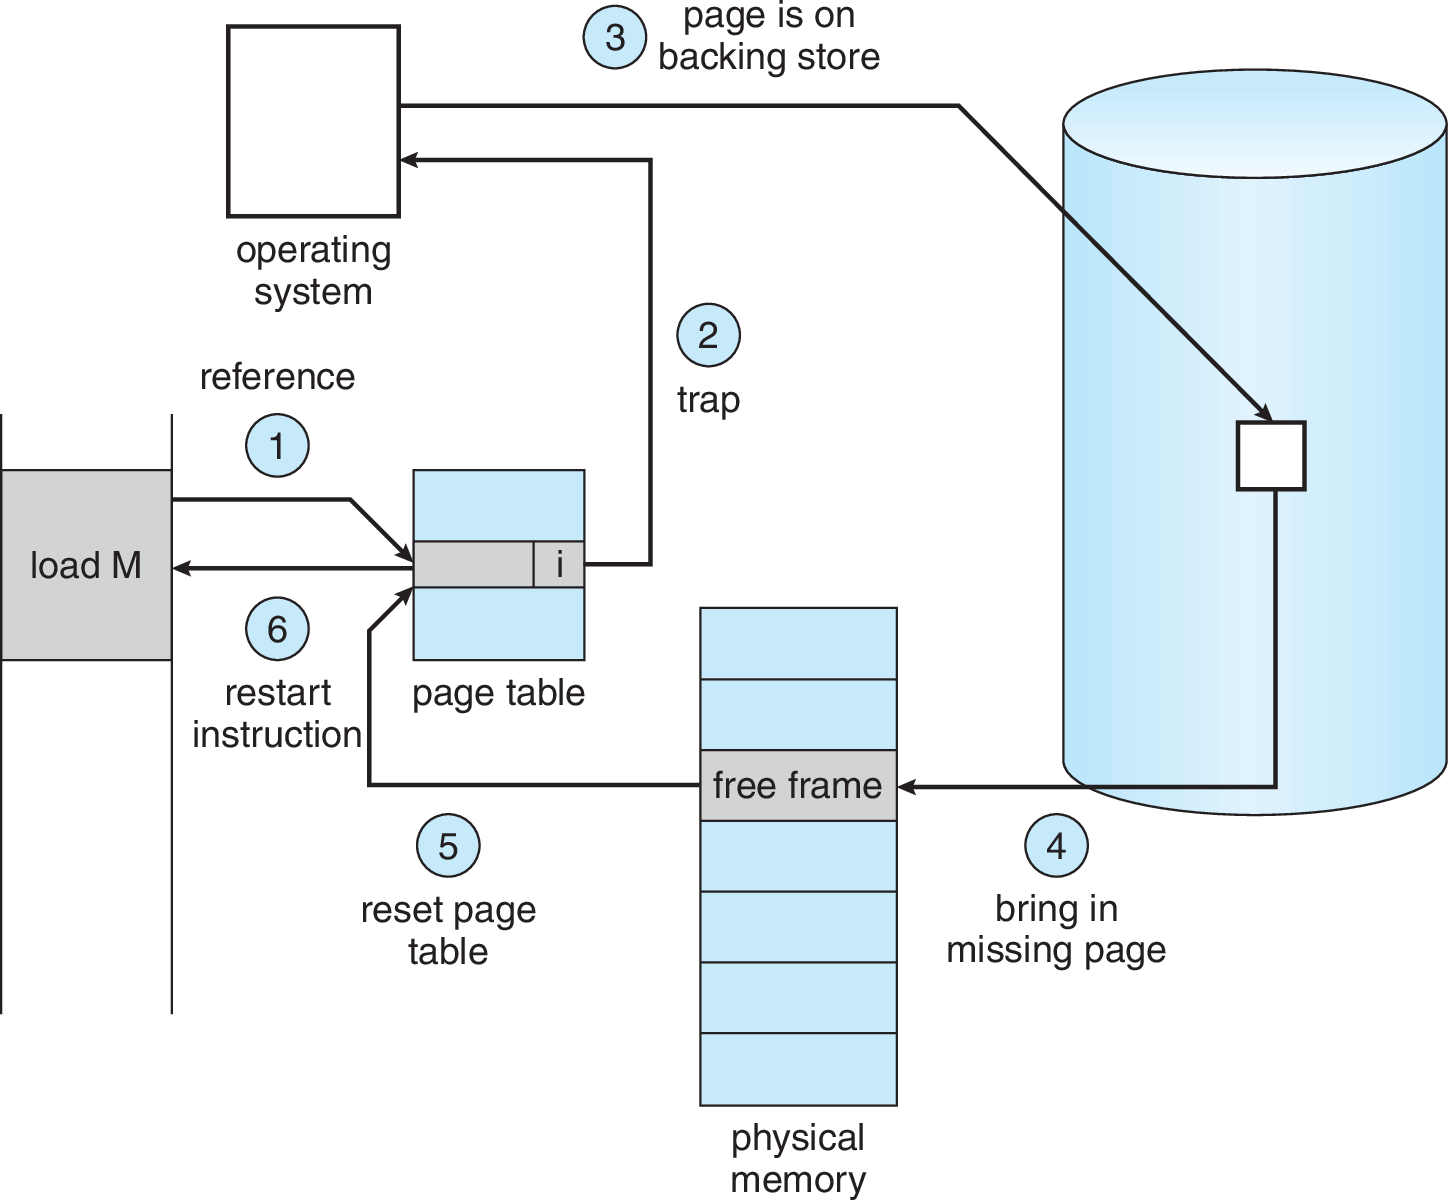
\includegraphics[width=6cm]{figs/02-9_06.pdf}
  \end{center}

  \begin{itemize}
    \item Proceso podría empezar con una única página en memoria: {\bf paginación por demanda pura}
  \end{itemize}

\end{frame}
%---------------------------------------------------------------------
\begin{frame}
  \frametitle{Paginación por demanda}

  Rendimiento de la paginación por demanda
  \begin{itemize}
    \item $p$, probabilidad de {\em page fault}
    \item $t_{ma}$, tiempo de acceso a memoria, $\sim 200 \times 10^{-9}s$
    \item $t_{pf}$, tiempo generado por {\em page fault}
  \end{itemize}
  
  \onslide<2->{
  Tiempo efectivo de acceso a memoria, $t_e$
  \[ t_e = (1-p) \times t_{ma} + p \times t_{pf} \]
  }
  
  \onslide<3->{
  Con $t_{pf} = 8 \text{ms}$:
  \[ t_{e} = 200 + 7999800 p \]
  }
  
  \onslide<4->{  
  Si queremos que la degradación no sea mayor a $10\%$:
  \[ 220 > 200 + 7999800p \Rightarrow p < 0.0000025 \]
  }
\end{frame}
%---------------------------------------------------------------------
\subsection{{\em Copy-on-Write}}

\begin{frame}
  \frametitle{{\em Copy-on-Write}}

  Al hacer un {\tt fork()} se {\em copia} la memoria del padre al hijo.
  
  \begin{itemize}
    \item ¿Y si el hijo no escribe en su memoria?
    \item ¿Y si el hijo hace inmediatemente {\tt exec()}?
  \end{itemize}
  
  Estrategia {\bf copy-on-write} mantiene las páginas del padre como
  {\em región compartida para el hijo}
  
  \begin{center}
    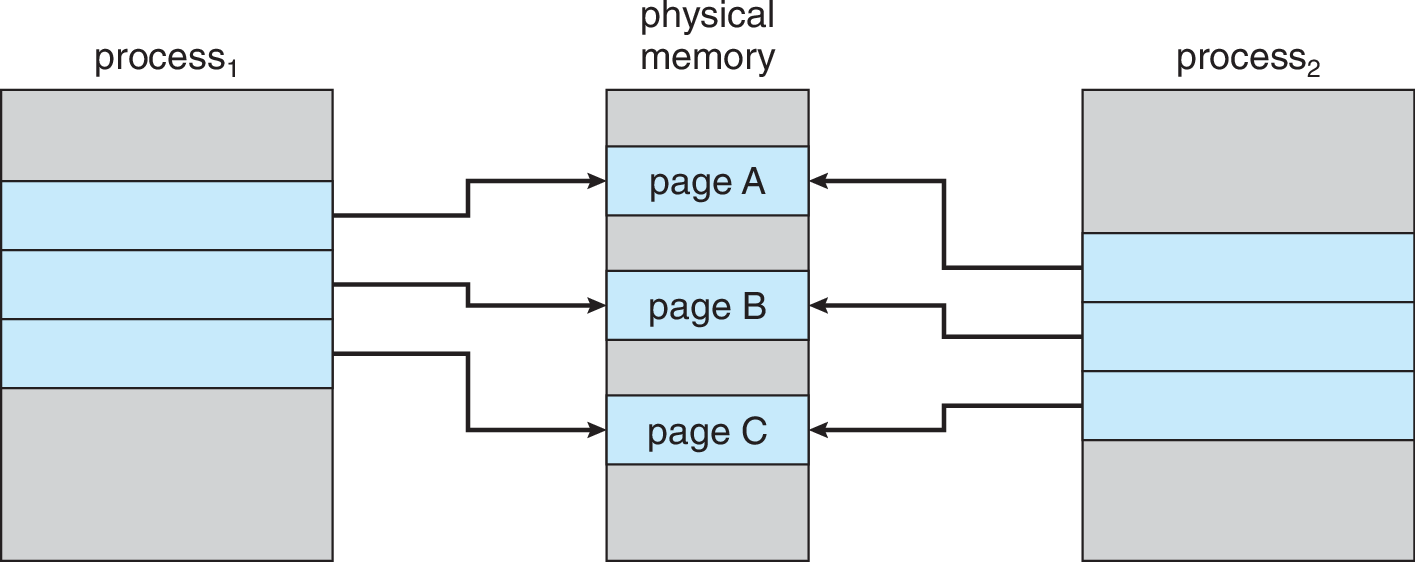
\includegraphics[width=5.5cm]{figs/02-9_07.pdf}
    \,\,\,\,\,\,
    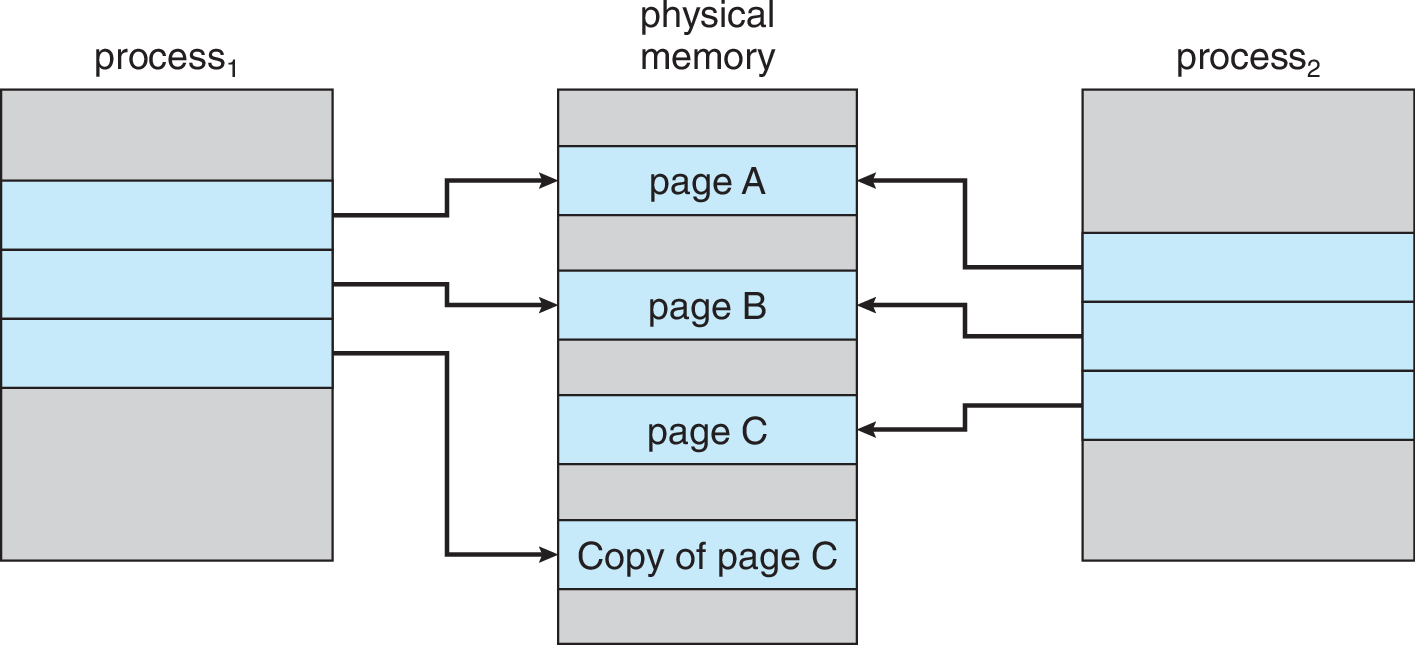
\includegraphics[width=5.5cm]{figs/02-9_08.pdf}
  \end{center}

  Instrucción {\tt vfork()} implementa {\tt fork} sin copia de páginas (ni con {\em copy-on-write})
  
\end{frame}

%---------------------------------------------------------------------
\subsection{Reemplazo de páginas}

\begin{frame}
  \frametitle{Reemplazo de páginas}

  Si sólo se carga la mitad de la memoria de un proceso, podemos cargar
  más en memoria $\to$ más multiprogramación

  Si no hay más espacio en memoria, se debe pasar a {\em swap} una de las páginas
  actualmente asignadas.

  \begin{center}
    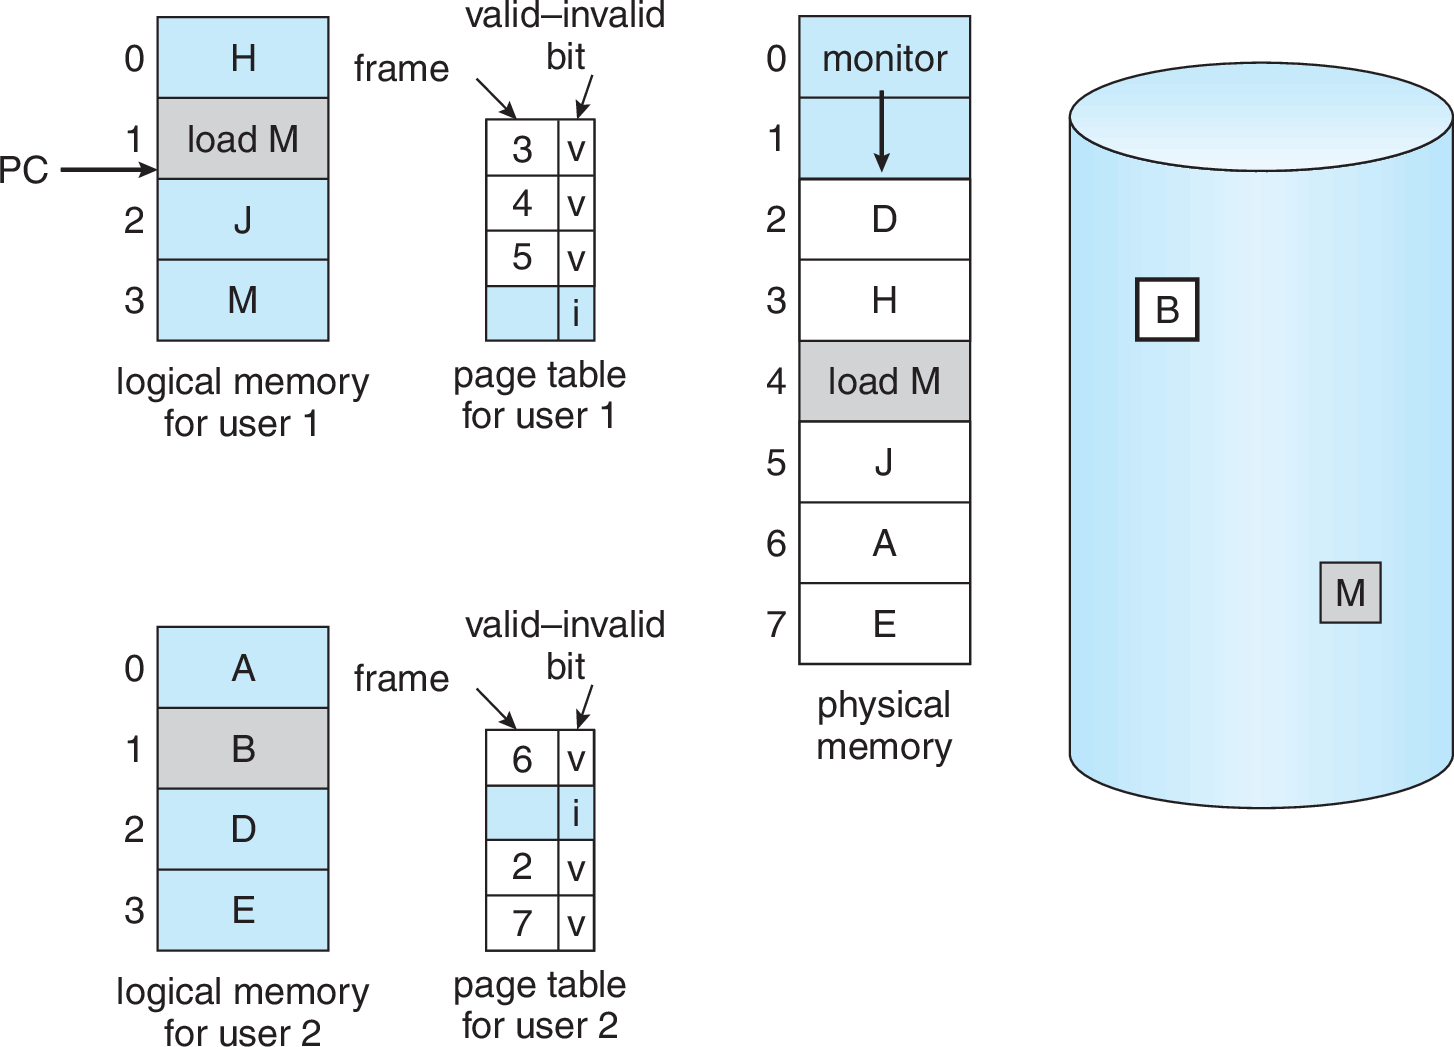
\includegraphics[width=7cm]{figs/02-9_09.pdf}
  \end{center}
  
  

\end{frame}

%---------------------------------------------------------------------
\begin{frame}
  \frametitle{Reemplazo de páginas}

  Sistema Operativo necesita {\bf reemplazar} una página existente,
  hacer {\em swap} y cargar otra

  \begin{center}
    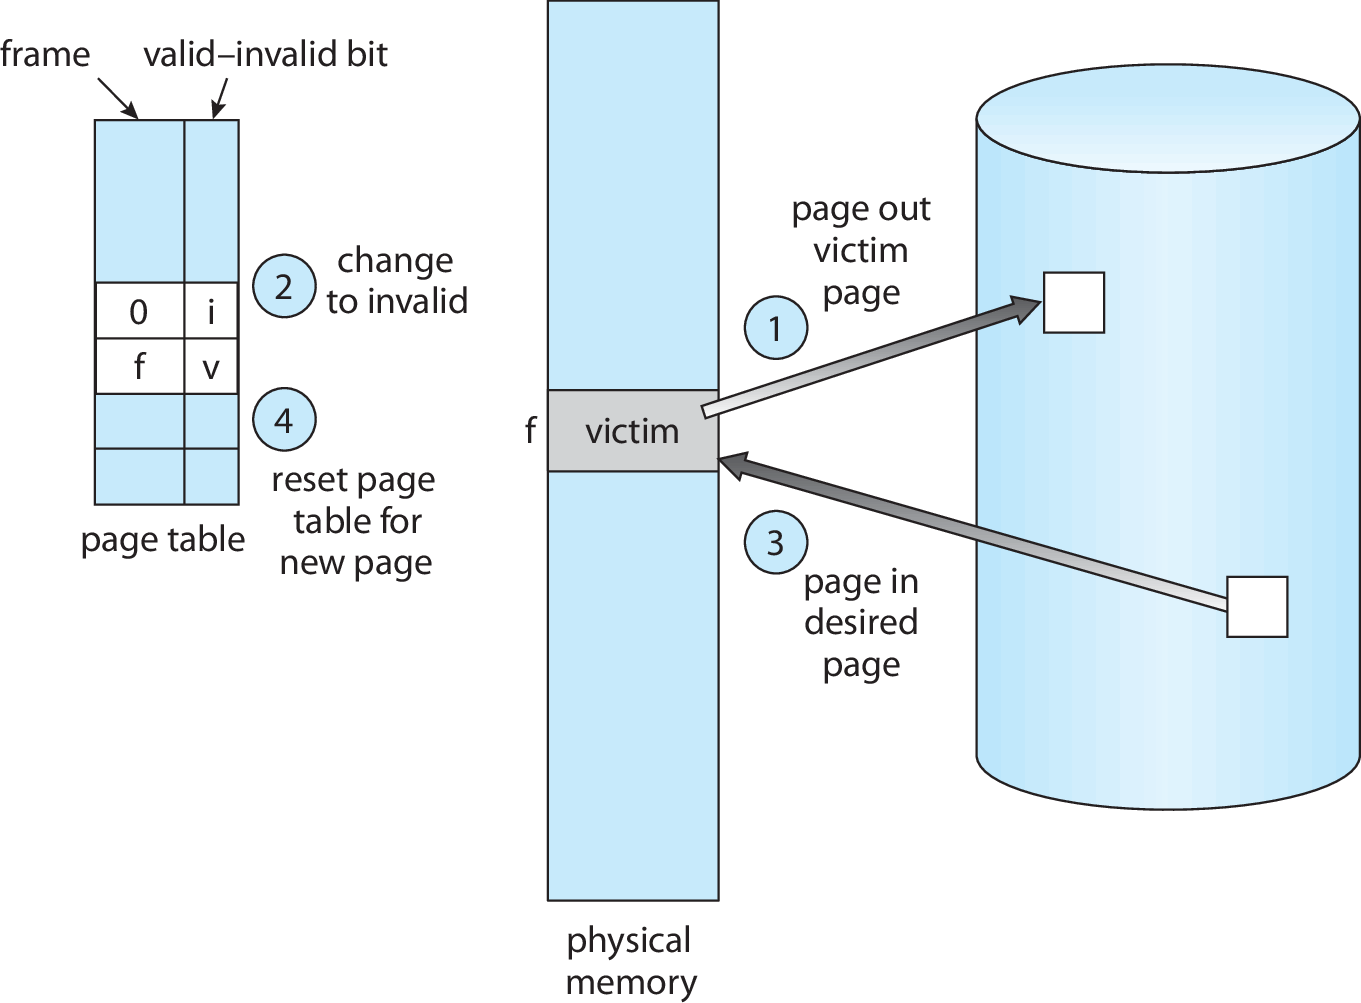
\includegraphics[width=7cm]{figs/02-9_10.pdf}
  \end{center}

  Algoritmos para elegir una página {\em víctima}  
  

\end{frame}
%---------------------------------------------------------------------
\begin{frame}
  \frametitle{Reemplazo de páginas}

  \begin{center}
    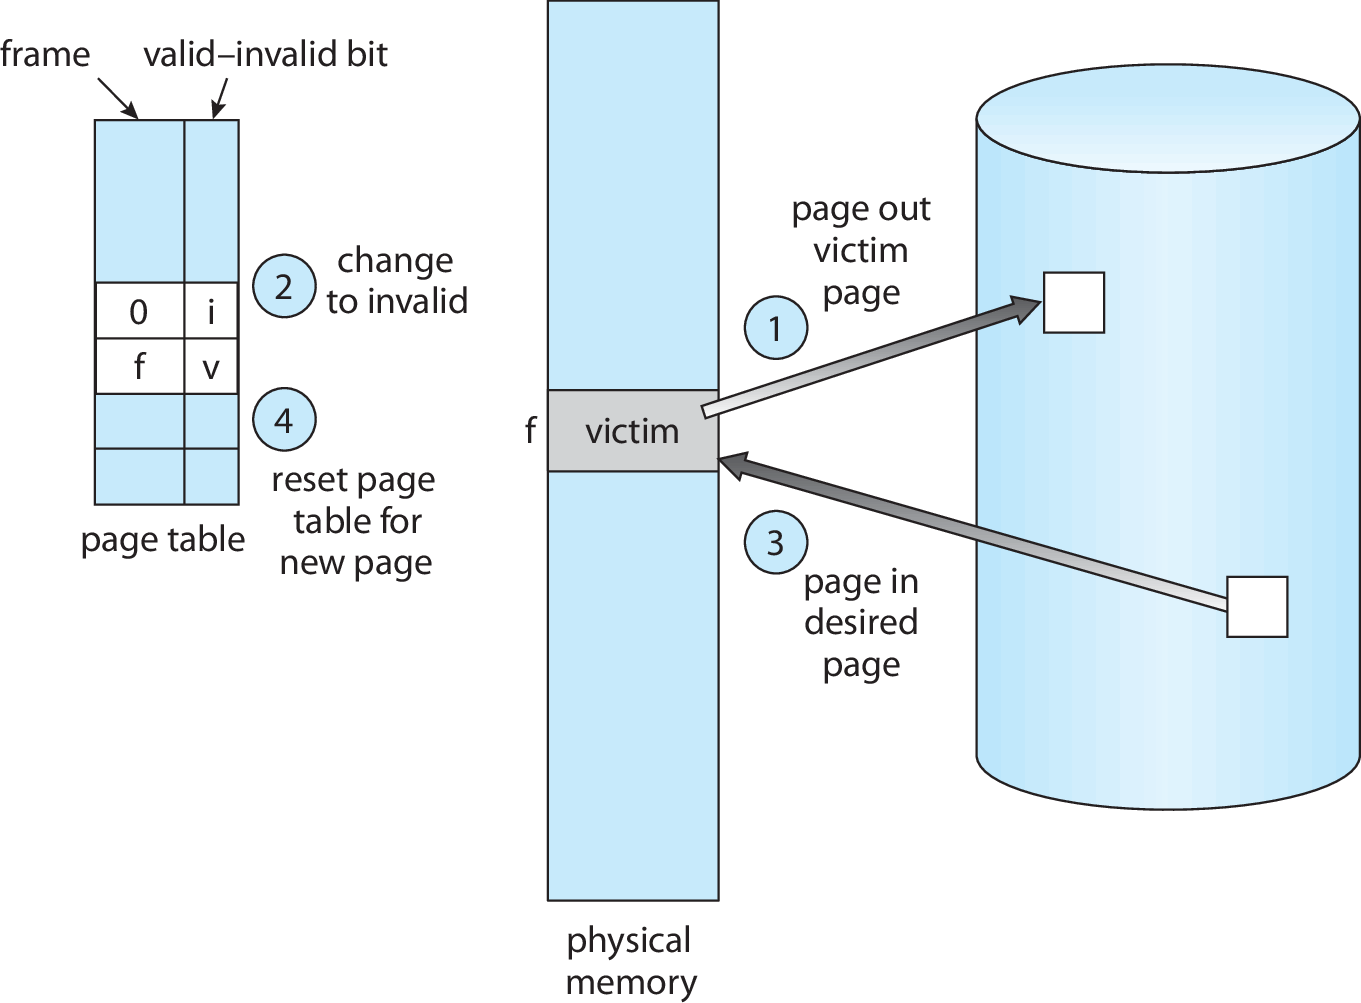
\includegraphics[width=6cm]{figs/02-9_10.pdf}
  \end{center}

  Dos transferencias de páginas (pasos 1 y 3)
  \begin{itemize}
    \item Páginas que no han sido modificadas no necesitan escribirse
          a disco
    \item {\bf Modify bit} o {\bf Dirty bit} indican si la página ha sido modificada
          desde la última vez que se cargó
    \item Páginas {\em read-only} nunca modifican su {\bf dirty bit}
  \end{itemize}

\end{frame}

%---------------------------------------------------------------------
\begin{frame}
  \frametitle{Reemplazo de páginas}

  Algoritmos para decidir {\em qué página reemplazar}
  \begin{itemize}
    \item ¿Cuál es mejor?
    \item Uno que genere pocos {\em page faults}
  \end{itemize}
  
  Comparables usando una misma secuencia de acceso a memoria
  \begin{itemize}
    \item Ej: Con esta secuencia de accesos a memoria
      \begin{itemize}
        \item 0145, 0400, 0102, 0670, 0110, 0672, 0112, 0198, 0153, 0602, 0170
      \end{itemize}
    \item Y con páginas que almacenen 100 direcciones, la secuencia de acceso es:
      \begin{itemize}
        \item 1,4,1,6,1,6,1,6,1
      \end{itemize}
  \end{itemize}

\end{frame}

%---------------------------------------------------------------------
\begin{frame}
  \frametitle{Reemplazo de páginas}

  \begin{center}
    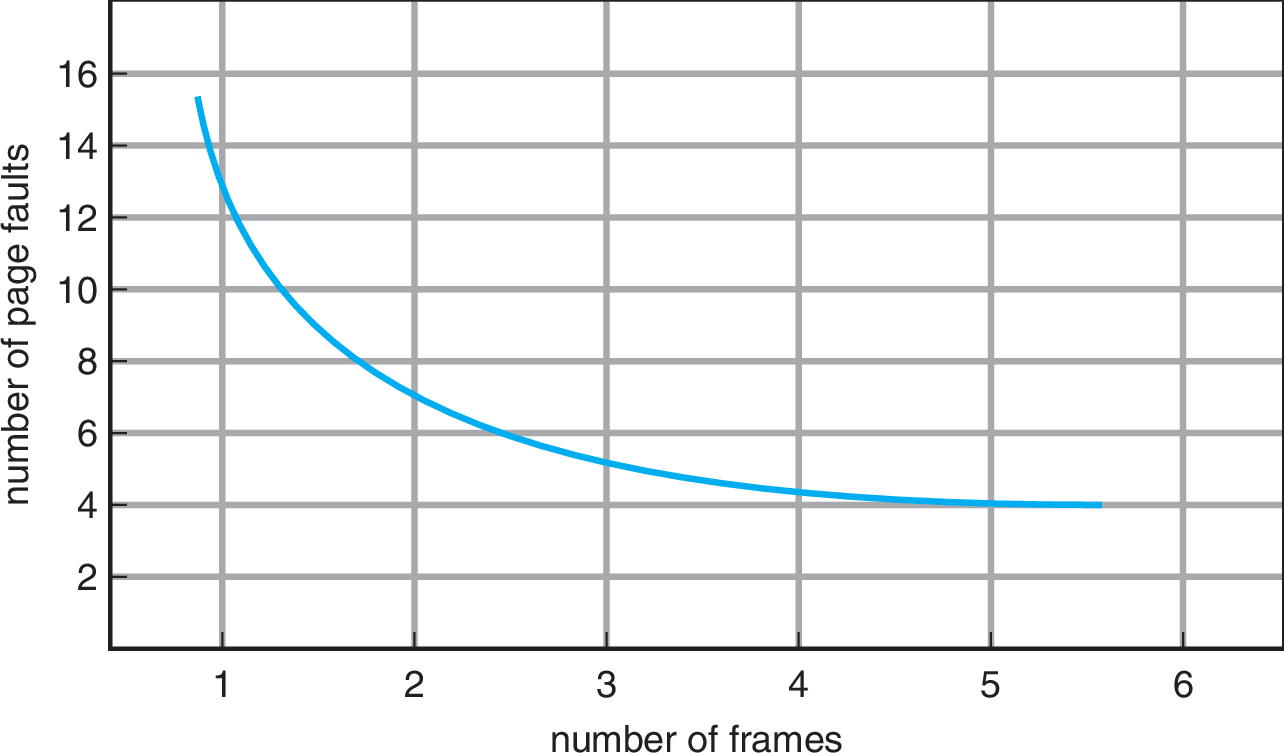
\includegraphics[width=6cm]{figs/02-9_11.pdf}
  \end{center}
  
  Tasa de {\em page faults} también depende de la cantidad de {\em frame} disponibles
  
\end{frame}

%---------------------------------------------------------------------
\begin{frame}
  \frametitle{Reemplazo FIFO}

  \begin{block}{{\bf FIFO}}
    Reemplazar la página que fue cargada hace más tiempo
  \end{block}

  \begin{center}
    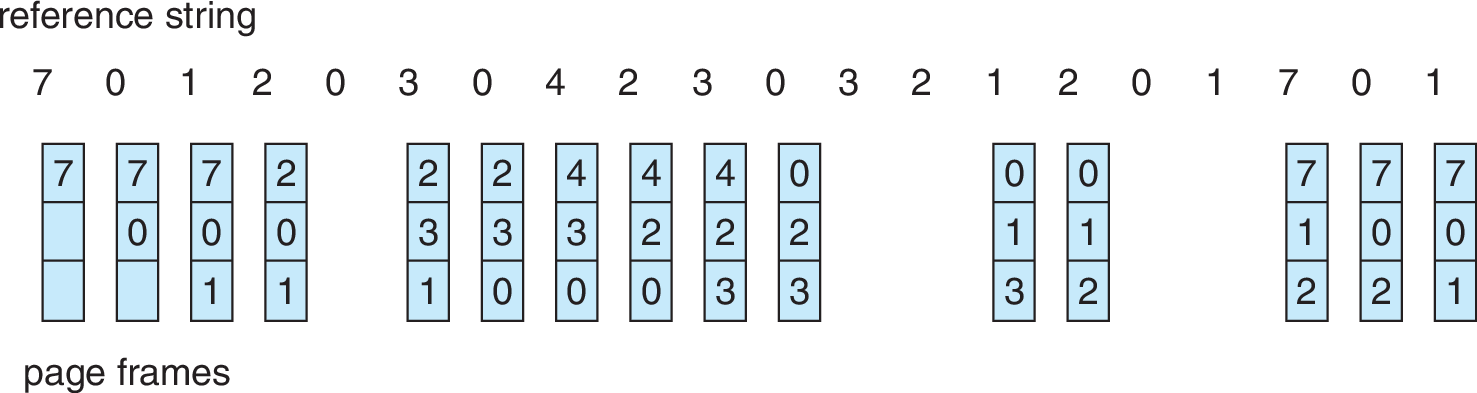
\includegraphics[width=10cm]{figs/02-9_12.pdf}
  \end{center}

  Se reemplaza la página más antigua en haber sido cargada
  \begin{itemize}
    \item +Fácil de implementar
    \item -Compartamiento impredecible
  \end{itemize}
\end{frame}

%---------------------------------------------------------------------
\begin{frame}
  \frametitle{Reemplazo FIFO}

  Aumentar la cantidad de {\em frames} debe disminuir la cantidad de {\em page faults}
  
  \begin{itemize}
    \item Ejemplo. Secuencia 1,2,3,4,1,2,5,1,2,3,4,5
    \item Con 3 frames genera 9 {\em page faults}
    \item Con 4 frames genera 10 {\em page faults} (¿?)
  \end{itemize}
  
  \begin{center}
    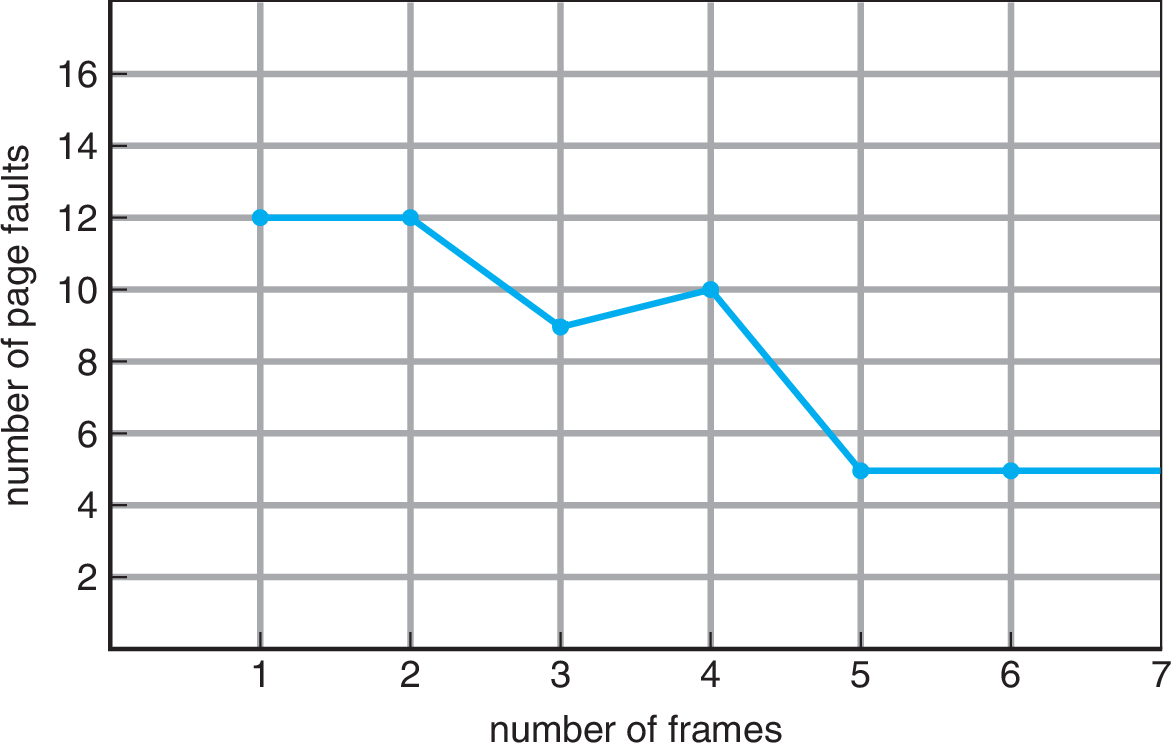
\includegraphics[width=5.5cm]{figs/02-9_13.pdf}
  \end{center}

  Este problema se conoce como {\bf anomalía de Bélády}\footnote{Planteada por el húngaro László Bélády, 1969} 

\end{frame}

%---------------------------------------------------------------------
\begin{frame}
  \frametitle{Reemplazo Óptimo}

  \begin{block}{{\bf OPT} ó {\bf MIN}}
    Reemplazar la página que no será usada por mayor tiempo
  \end{block}

  No sufre la anomalía de Bélády.

  \begin{center}
    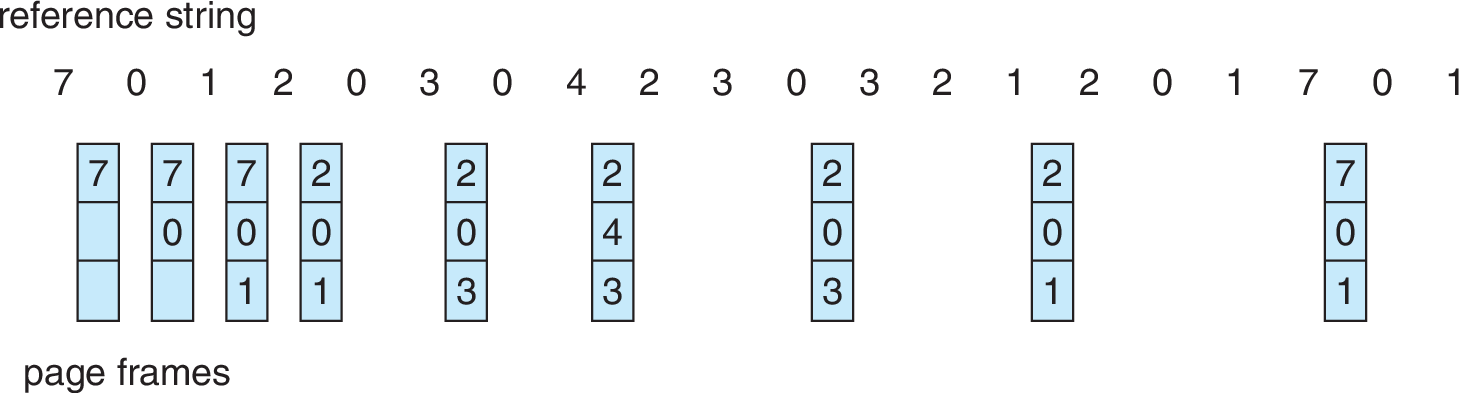
\includegraphics[width=8cm]{figs/02-9_14.pdf}
  \end{center}

  \begin{itemize}
    \item +Óptimo
    \item -Difícil de implementar, pues requiere conocimiento futuro (como SJF)
  \end{itemize}

\end{frame}
%---------------------------------------------------------------------
\begin{frame}
  \frametitle{Reemplazo LRU ({\em Least Recently Used})}
  \framesubtitle{Si no puedes obtener el óptimo, aproxímalo}

  \begin{block}{{\bf LRU}}
    Reemplazar la página que no ha sido usada por más tiempo
  \end{block}
  
  \begin{center}
    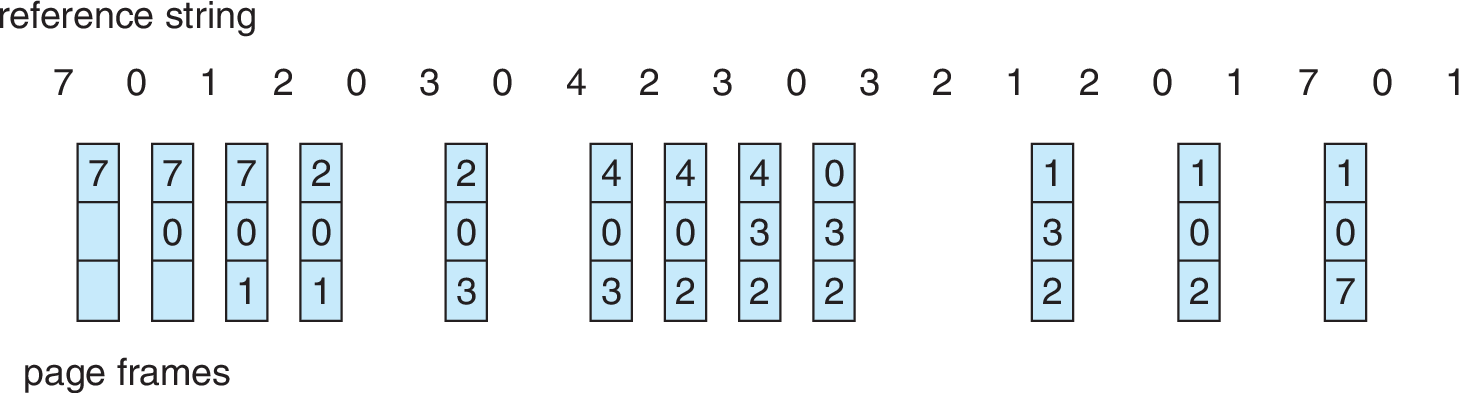
\includegraphics[width=8cm]{figs/02-9_15.pdf}
  \end{center}

  Parece un buen compromiso. ¿Cómo implementarlo?
  \begin{itemize}
    \item Contadores, actualizado con valor de {\em timer}
    \item {\em Stack}, el último acceso avanza al tope del {\em stack}
  \end{itemize}

  En cualquier caso se requiere ayuda de {\em hardware}
\end{frame}
%---------------------------------------------------------------------
\begin{frame}
  \frametitle{Aproximación a LRU}

  Si no hay soporte de {\em hardware}, se puede aproximar el comportamiento de LRU
  
  \begin{itemize}
    \item {\bf Reference bit} se marca para indicar páginas referenciadas
    \item Permite determinar qué páginas se han usado y cuáles no (sin orden)
  \end{itemize}

  Una técnica para incorporar orden:
  \begin{itemize}
    \item 8-bit reference ({\em reference byte}) funcionan como ``bit de historia''
    \item A intervalo $r$ ($\sim 100$ms) se hace {\em right shift}
          del {\em reference bit}
    \item Frame con mayor {\em reference byte} es el usado más recientemente    
  \end{itemize}
  
  Valores pueden no ser únicos. Entre ellos se decide de manera FIFO.
  
\end{frame}
%---------------------------------------------------------------------
\begin{frame}
  \frametitle{Aproximación a LRU: Algoritmo de segunda oportunidad}
  \framesubtitle{Otra oportunidad, otra oportunidad, \ldots}

  Inicialmente, algoritmo FIFO, ordenado por tiempo de carga
  \begin{itemize}
    \item Al ser elegida, se observa su {\em reference bit}
      \begin{itemize}
        \item Reference bit 0: se reemplaza
        \item Reference bit 1: 2da oportunidad. Se cambia a 0, se establece tiempo de carga al tiempo actual, 
              y se pasa a la siguiente página
      \end{itemize}
  \end{itemize}

  \begin{center}
    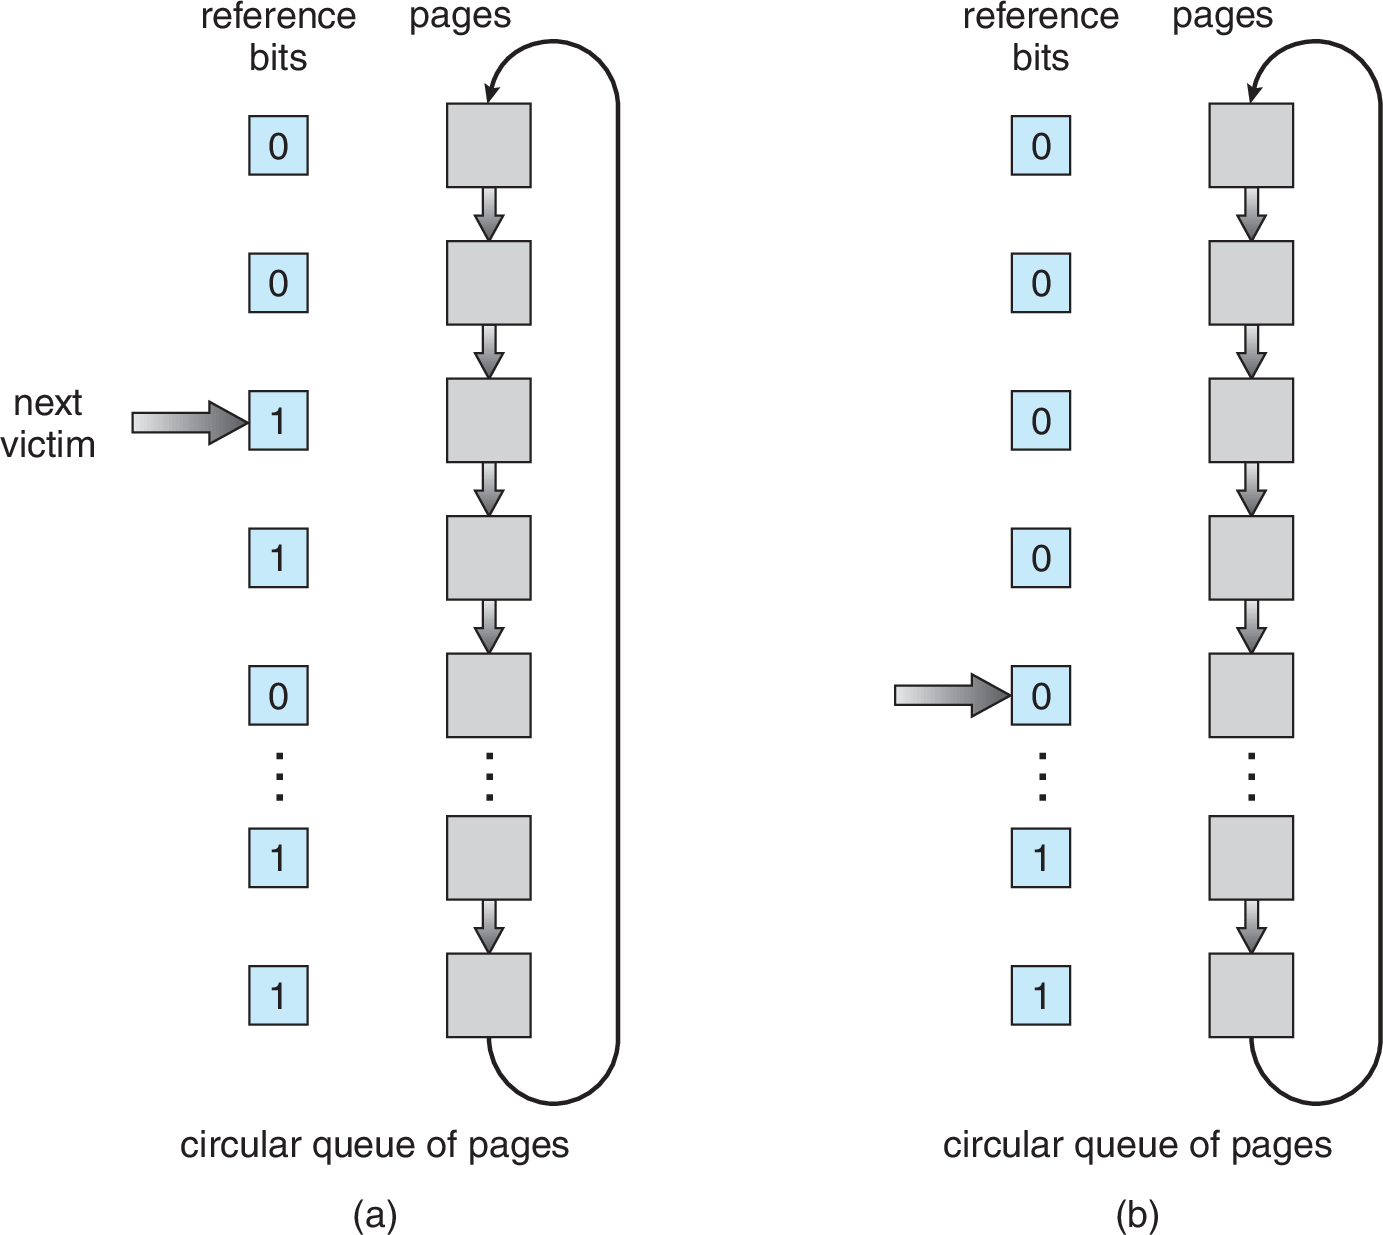
\includegraphics[width=4cm]{figs/02-9_17.pdf}
  \end{center}
  
  ¿Qué pasa si todos los bit están marcados como 1?

\end{frame}
%---------------------------------------------------------------------
\begin{frame}
  \frametitle{Aproximación a LRU: Segunda oportunidad mejorada}

  2da oportunidad considerando el par ({\em reference bit}, {\em dirty bit})
  
  \begin{itemize}
    \item (0,0), no usado recientemente ni modificada
      \begin{itemize}
        \item Buena víctima
      \end{itemize}
    \item (0,1), no usada recientemente, pero modificada
      \begin{itemize}
        \item Casi buena víctima. Requiere escribirla.
      \end{itemize}
    \item (1,0), recientemente usada, pero no modificada
      \begin{itemize}
        \item Probablemente será leída pronto
      \end{itemize}
    \item (1,1), recienemente usada, y modificada
      \begin{itemize}
        \item Probablemente será leída pronto
      \end{itemize}
  \end{itemize}

\end{frame}

%---------------------------------------------------------------------
\begin{frame}
  \frametitle{Otros algoritmos}
  
  Con contador de accesos (costoso de implementar)
  \begin{itemize}
    \item {\bf Least Frequently Used}. Una página muy accedida debe tener alto contador.
       \begin{itemize}
         \item ¿Y si se usó solo al inicio?
         \item Se puede complementar haciendo {\em shift} del contador periæodicamente
       \end{itemize}
    \item {\bf Most Frequently Used}. La página que tiene pocos accesos probablemente fue cargada recientemente
          y aún no ha sido muy usada
  \end{itemize}
\end{frame}

%---------------------------------------------------------------------
\subsection{Asignación de {\em Frames} y {\em Thrashing}}

\begin{frame}
  \frametitle{Asignación de {\em Frames}}

  La pregunta: ¿cuántos {\em frames} asignar a cada proceso?
  
  {\bf Mínimo}
  \begin{itemize}
    \item Puede ser definido por la arquitectura
    \item O bien, depender de la cantidad de direcciones referenciables en una instrucción
      \begin{itemize}
        \item {\tt load r1, 0x0160}. Dos frames: para la instrucción y para la dirección.
        \item Más complejo cuando se permiten indirecciones
      \end{itemize}
  \end{itemize}
  
  {\bf Máximo}
  \begin{itemize}
    \item ¿Cómo dividir $m$ {\em frames} entre $n$ procesos?
  \end{itemize}

\end{frame}

%---------------------------------------------------------------------
\begin{frame}
  \frametitle{Asignación de {\em Frames}}

  $m$ {\em frames} y $n$ procesos
  \begin{itemize}
    \item {\bf Asignación equitativa}: $\lfloor m/n \rfloor$ a cada uno. 
    \item {\bf Asignación proporcional}: sea $s_i$ el tamaño de la memoria virtual del proceso $p_i$,
          cada proceso recibe $a_i$ {\em frames}: 
          \[ a_i = \frac{s_i}{\sum{s_i}} \times m \]
          Proporción también puede estar relacionada a la prioridad del proceso
          
  \end{itemize}

\end{frame}

%---------------------------------------------------------------------
\begin{frame}
  \frametitle{{\em Thrashing}}

  Cada {\em page fault} genera tráfico entre disco y memoria de {\em al menos} una página.
  
  \vspace{1em}

  \onslide<2->{Con alta tasa de {\em page fault} el sistema gasta más tiempo copiando {\em frames}
               entre disco y memoria}
  \vspace{1em}        

  \onslide<3->{Se produce {\bf thrashing}}

\end{frame}
%---------------------------------------------------------------------
\begin{frame}
  \frametitle{{\em Thrashing}}

  \begin{center}
    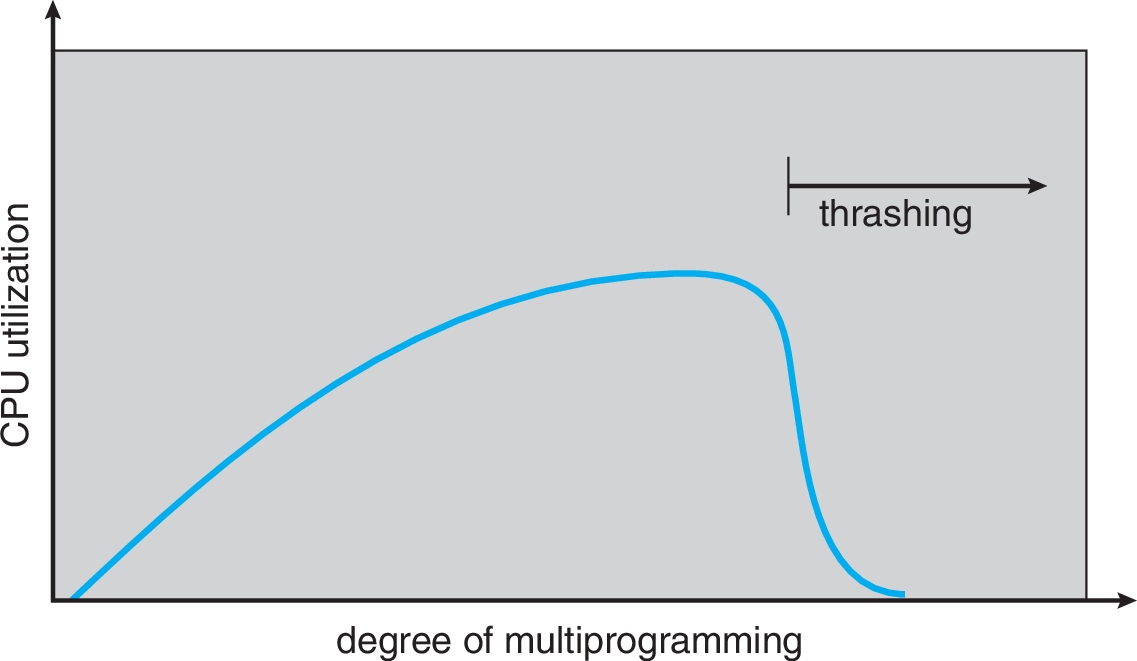
\includegraphics[width=6cm]{figs/02-9_18.pdf}
  \end{center}

  \begin{itemize}
    \item Baja utilización de CPU
    \item {\em Scheduler} incrementa nivel de multiprogramación
    \item Procesos nuevos requieren {\em frames}.
    \item S.O. quita {\em frames} a procesos en ejecución
    \item Procesos en ejecución aumentan su tasa de {\em page fault}
    \item S.O. gasta más tiempo cargando {\em frames}
    \item Baja utilización de CPU
  \end{itemize}

\end{frame}

%---------------------------------------------------------------------
\begin{frame}
  \frametitle{Localidad de referencia}

  Estrategia para evitar {\em thrashing}: aprovechar la {\bf localidad de referencia}
  
  \begin{itemize}
    \item Teoría: procesos saltan de una localidad a otra
    \item Referencias se dan principalmente en una localidad de memoria y,
          con baja frecuencia, saltan a otro localidad
  \end{itemize}
  
  \begin{center}
    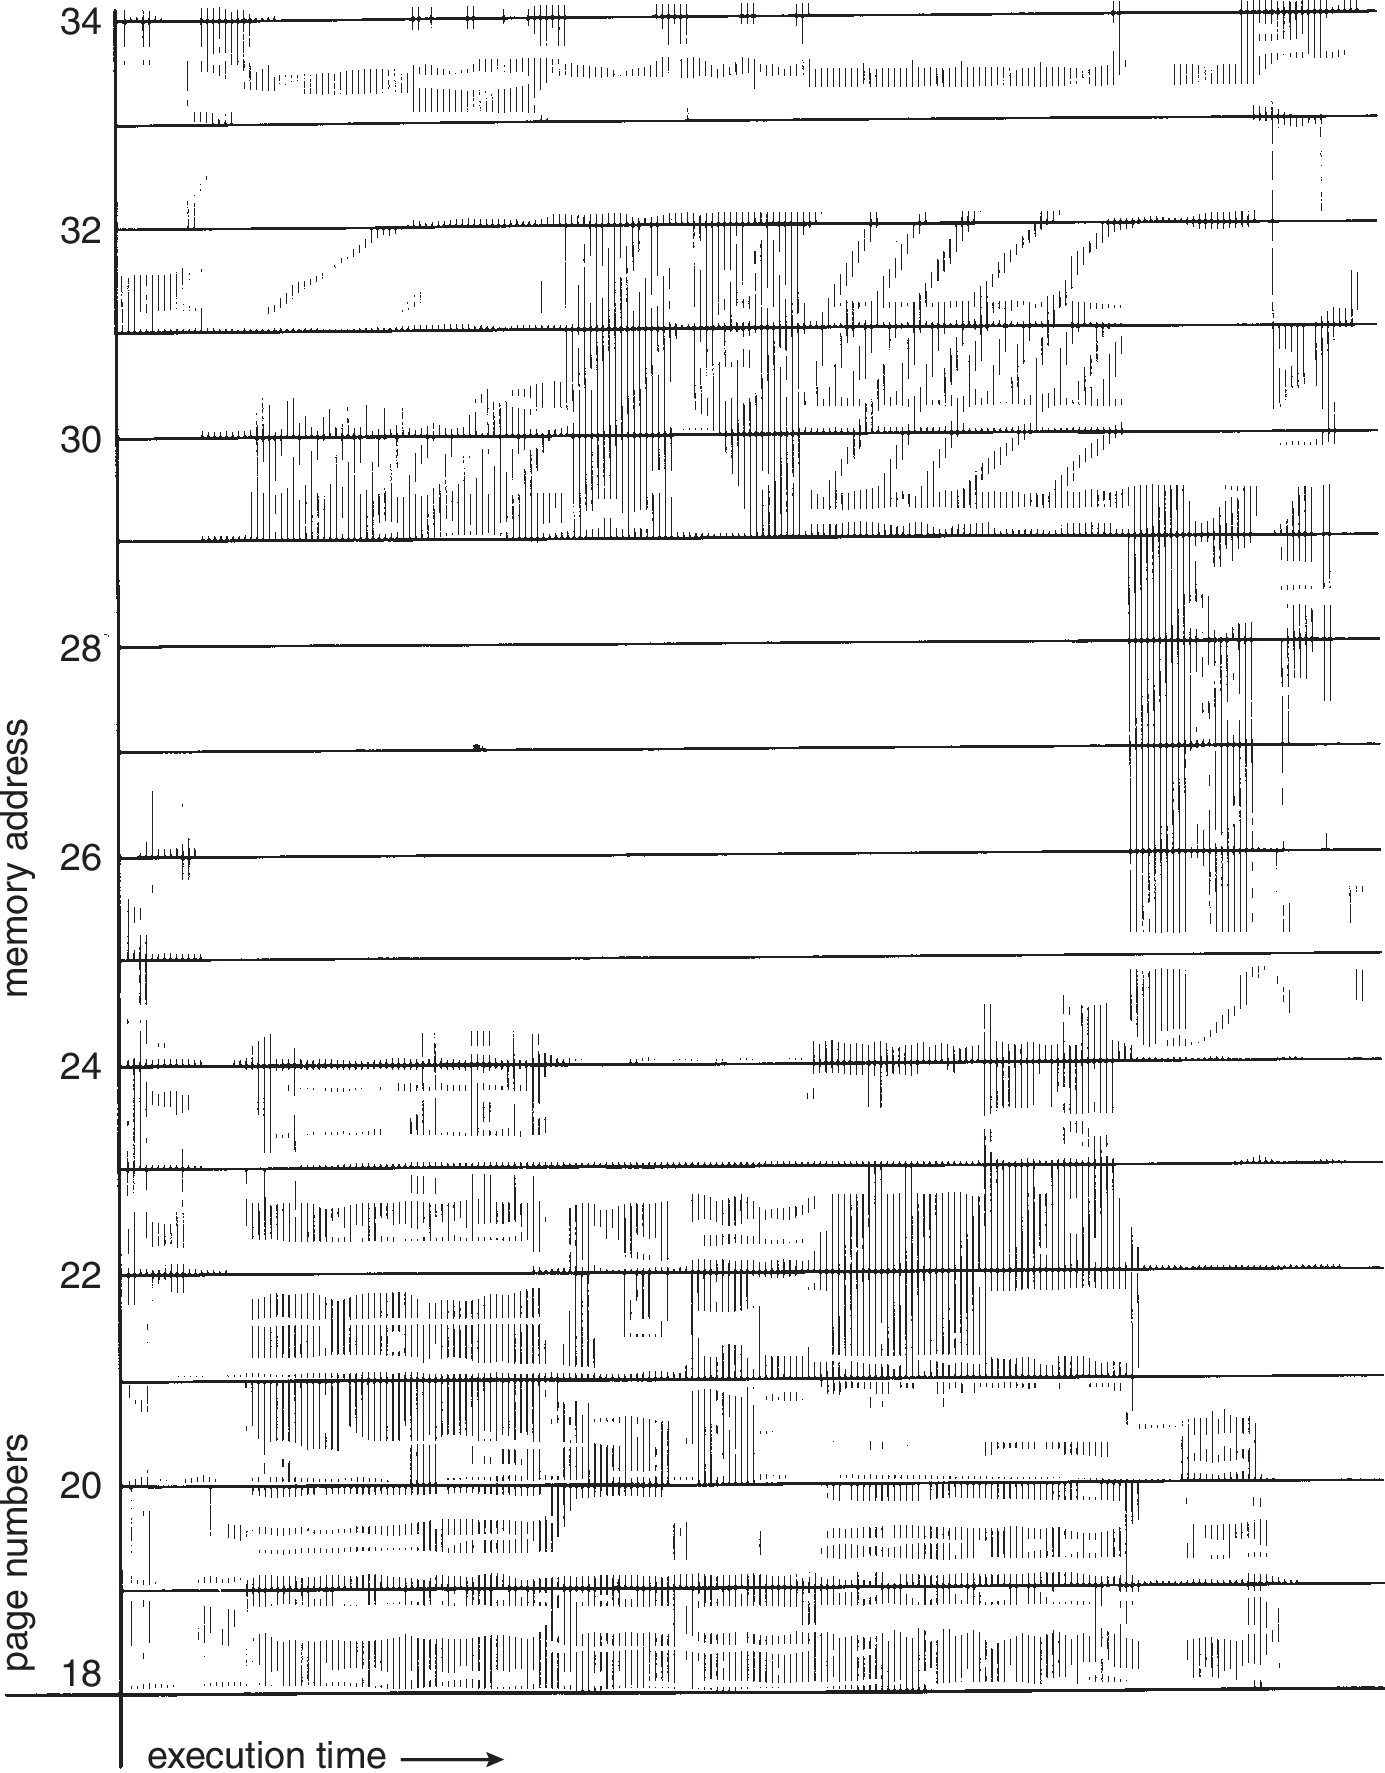
\includegraphics[width=4cm]{figs/02-9_19.pdf}
  \end{center}


\end{frame}

%---------------------------------------------------------------------
\begin{frame}
  \frametitle{Modelo de {\em Working Set}}

  \begin{block}{{\bf Working Set}}
    Conjunto de páginas usadas en los últimos $\Delta$ accesos
  \end{block}

  \begin{center}
    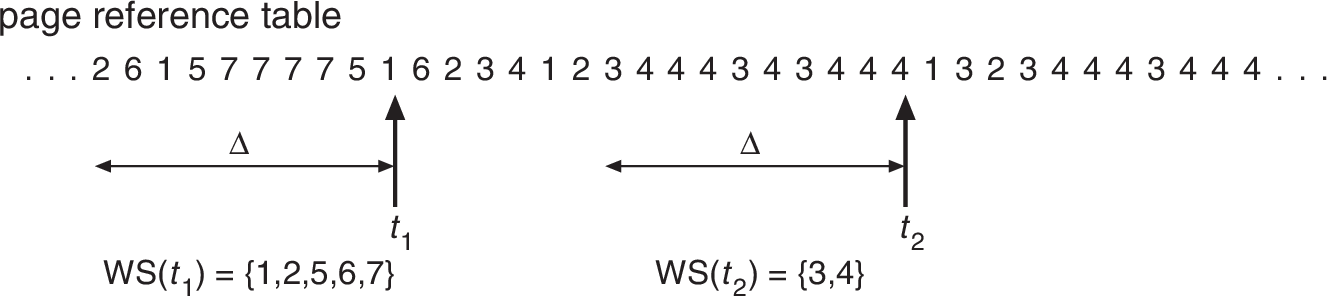
\includegraphics[width=9cm]{figs/02-9_20.pdf}
  \end{center}

  $\Delta$ determina el tamaño del {\em working set} del proceso $i$: $\text{WSS}_i$
  
  \vspace{1em}
  
  Demanda por páginas: $D=\sum{\text{WSS}_i}$
  
  \vspace{1em}
  
  Si hay $m$ frames, y $D > m$, entonces habrá {\em thrashing}

\end{frame}

%---------------------------------------------------------------------
\begin{frame}
  \frametitle{Modelo de {\em Working Set}}
  \framesubtitle{¿Cómo implementarlo?}

  Aprovechar los {\em reference bit}
  
  \begin{itemize}
    \item Observar {\em reference bit} a intervalos regulares, cada $R$ referencias
    \item {\em Reference bit} se copian y se borran
    \item En la siguiente observación se comparan los valores copiados
          y los nuevos {\em reference bit}.
    \item Páginas modificadas se mantienen dentro del {\em working set}
  \end{itemize}
  Permite aproximar el {\em working set}, a menor costo que analizar todas las referencias

\end{frame}
%---------------------------------------------------------------------

\begin{frame}
  \frametitle{Resumen}

  \begin{itemize}
    \item Direccionamiento de memoria
      \begin{itemize}
        \item Transformaciones de dirección lógica a física
        \item Tipos de asignacioens: contigua, segmentada, paginada
      \end{itemize}
    \item Memoria Virtual
      \begin{itemize}
        \item Permite direccionar más memoria que la memoria física disponible
        \item Páginas se asignan a {\em frames} en la medida que se necesiten
        \item Si no hay {\em frames} disponibles se debe reemplazar alguna página
        \item Reemplaza FIFO, OPT, LRU
        \item Cantidad de {\em frames} asignados a cada proceso debe ser el apropiado,
              de lo contrario se puede producir {\em thrashing}
      \end{itemize}
  \end{itemize}

\end{frame}
%---------------------------------------------------------------------
\end{document}